\documentclass[10pt,a4paper]{article}

\usepackage{setspace}
\usepackage{sectsty}
\usepackage{lipsum}
\usepackage{xcolor}
\usepackage[T1]{fontenc}
\usepackage{float}
\usepackage[utf8]{inputenc}
\usepackage{natbib}
\usepackage{graphicx}
\usepackage{pdflscape}
\usepackage{listings}
\usepackage{subcaption}
\usepackage{multirow}
\usepackage{tabularx} 
\usepackage{pdfpages}
\usepackage{fontspec}
\usepackage{xcolor}
\usepackage{listings}
\usepackage{titlesec}
\usepackage{layout}
\usepackage{amsmath}
\setcitestyle{square}


%FORMATAÇÃO DAS MARGENS, CABEÇALHO E RODAPÉ
\usepackage[a4paper,left=2.5cm,right=1.5cm,top=3cm,bottom=3cm,
            footskip = 30pt,
            headheight= -0.5cm,
            headsep=3cm
            ]{geometry}
%%            
\usepackage{stackengine,xcolor}
\usepackage{fancyhdr}
\usepackage{chngcntr}
\counterwithin{figure}{section}
\counterwithin{table}{section}
\counterwithin{equation}{section}

\fboxrule=2pt
\newcommand\cincludegraphics[2][]{%
  \setbox0=\hbox{\includegraphics[#1]{#2}}
  \abovebaseline[-0.5\ht0]{\includegraphics[#1]{#2}}}
\newcommand\dincludegraphics[2][]{%
  \setbox0=\hbox{\includegraphics[#1]{#2}}%
  \belowbaseline[+0.5\ht0]{\includegraphics[#1]{#2}}}
\usepackage{fancyhdr}
\usepackage{graphicx}
\usepackage{indentfirst}
\usepackage{hyphenat}
\hyphenation{refri-gerante}

\captionsetup{labelsep=endash}

\renewcommand\refname{Bibliografia}
\renewcommand{\figurename}{Figura}
\renewcommand\tablename{Tabela}
            
\defaultfontfeatures{Ligatures=TeX}
            
\renewcommand{\baselinestretch}{1.5}
        


            
% Turn on the style
\pagestyle{fancy}
% Clear the header and footer
\fancyhead{}
\fancyfoot{}


% Preenchendo cabeçalho
\fancyhf{}  
\lhead{\addstackgap[3pt]{
  \makebox[\dimexpr\textwidth-2\fboxsep-2\fboxrule\relax]{%
  \hspace*{-3.6cm} 
  \parbox[c]{10cm}{\textbf{\red{Graduação em Engenharia Mecânica\\
168041 - Instalações Termomecânicas 1}}\\
Prof. João Pimenta\\}\hfil
}}}
\chead{}
\rhead{\textbf{PROJETO}}
%%

\renewcommand{\headrulewidth}{0pt}
\renewcommand{\footrulewidth}{0pt}
\renewcommand{\thesection}{\arabic{section}}
%Modificando texto campo "Table of contents" para "Sumário" e modificando fonte para CALIBRI negrito
\renewcommand{\contentsname}{\fontspec{CALIBRIB.TTF}SUMÁRIO}
%Modificando de "list of figures" para "Lista de Figuras" e modificando fonte para CALIBRI negrito
\renewcommand{\listfigurename}{\fontspec{CALIBRIB.TTF}LISTA DE Figuras}
%Modificnado de "List of tables" para "Lista de tabelas" e modificando fonte para CALIBRI negrito
\renewcommand{\listtablename}{\fontspec{CALIBRIB.TTF}LISTA DE TABELAS}
%Inserindo rodapé do LAAR no lado esquerdo do rodapé
\lfoot{\addstackgap[3pt]{
  \makebox[\dimexpr\textwidth-2\fboxsep-2\fboxrule\relax]{%
  \hspace*{-4cm} 
  \cincludegraphics[scale=0.2]{Figuras/LAAR}\hfil 
  %\parbox[c]{1in}{Some text to go in the footer}\hfil
}}}
\rfoot{\thepage~}
\sectionfont{\fontsize{14pt}{10pt}\selectfont}
\subsectionfont{\fontsize{10pt}{10pt}\selectfont}
\setlength{\parindent}{1cm}


\begin{document}
%Definido Spranq_eco_sans como a fonte principal
\setmainfont{[spranq_eco_sans_regular.ttf]}

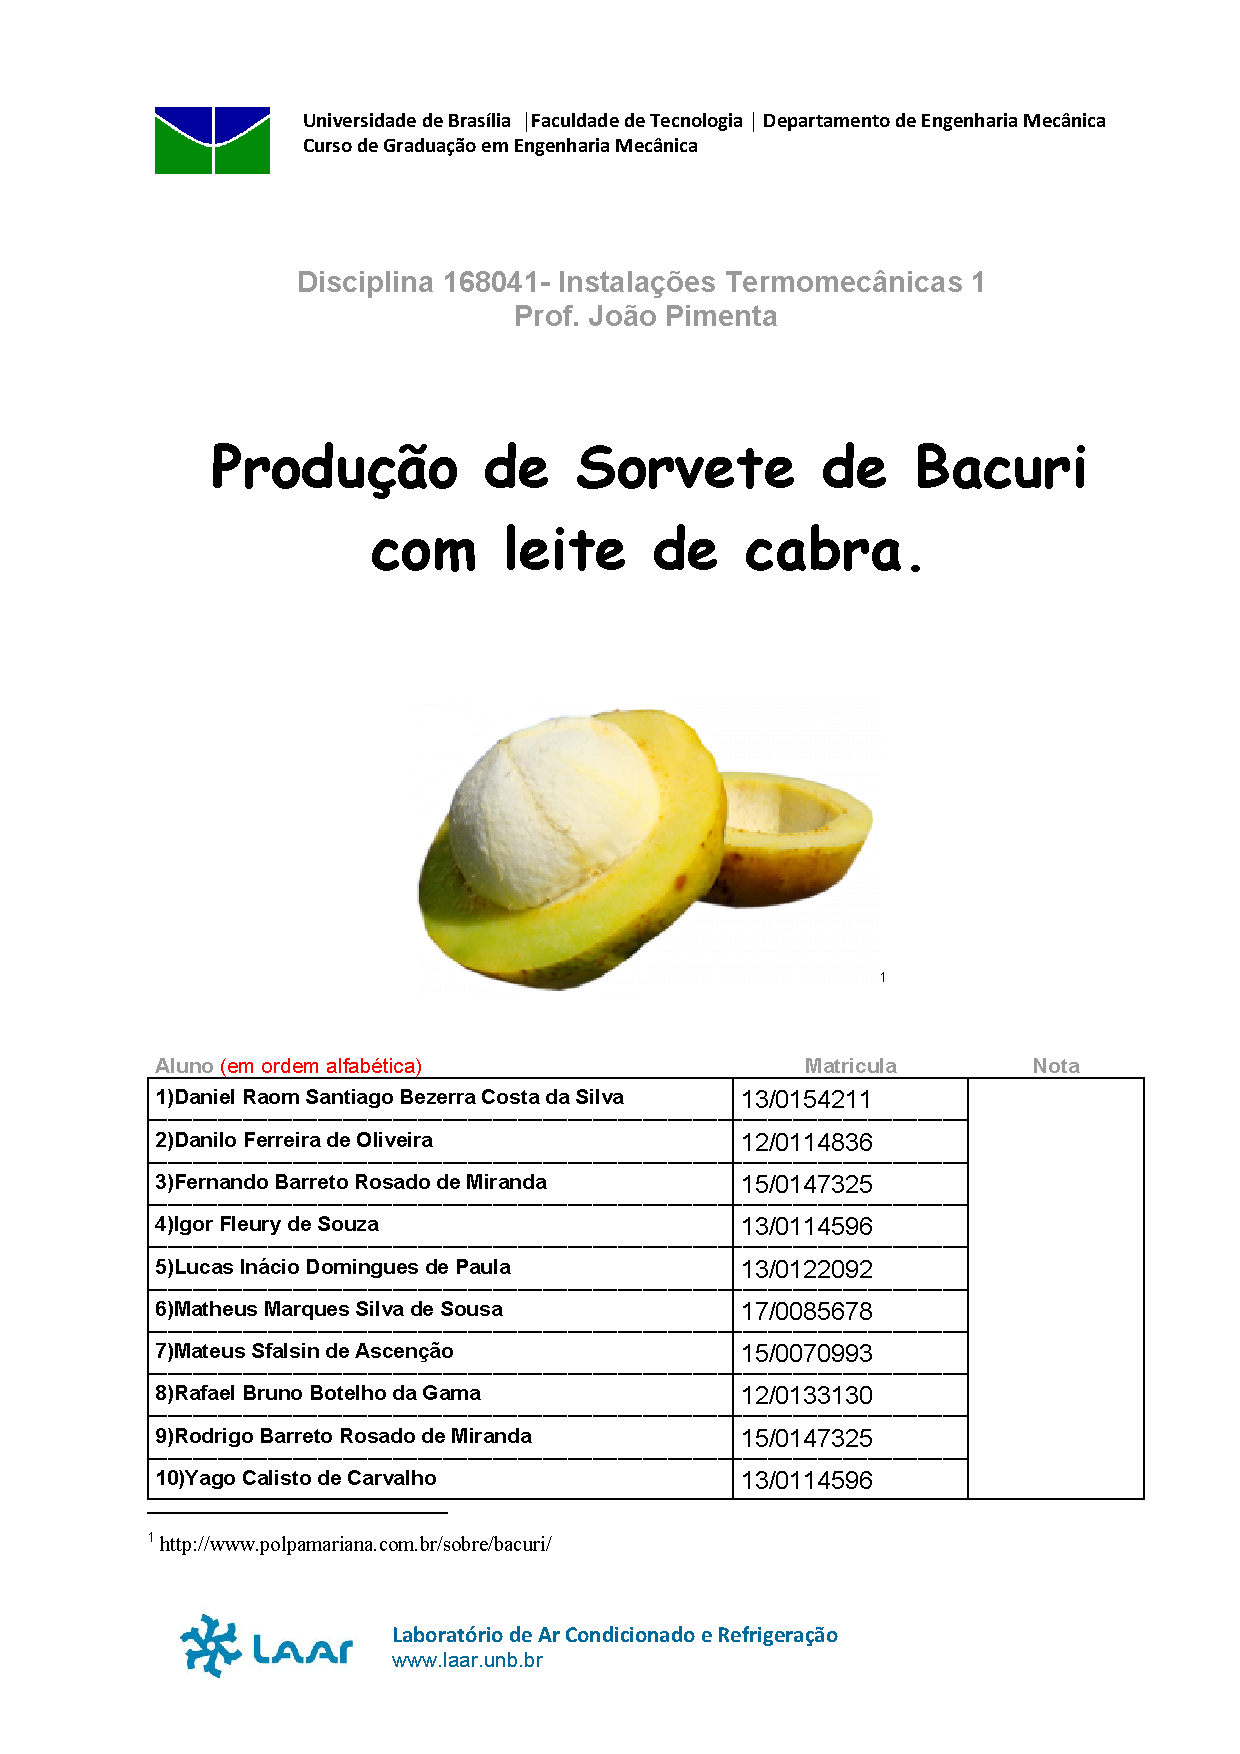
\includepdf{capa_insta1} 

\tableofcontents

\newpage
\listoffigures
\newpage
\listoftables


%INTRODUÇÃO

%NOTA, SEMPRE AO CRIAR SECTIONS E SUBSECTIONS utilizar este formato para modificar a fonte, caso contrário será utilizada a fonte padrão do corpo do texto.
\newpage

%INTRODUÇÃO%%%%%%%%%%%%%%%%%%%%%%%%%%%%%%%%%%%%%%%%%%%%%%%%%%%%%%%%%%%%%%%%%%%%%%%%%%%%%%%%%%%%%%%%%%%%%%%%%%%%%%%%%%%%%%%%%%%%%%%%%%%%%%%%%%%%%%%%%%%%%%%%%%%%%%%%%%%%%
\section{\fontspec{CALIBRIB.TTF}{ INTRODUÇÃO}}

\subsection{{\fontspec{Arial} Estado da arte}}

\par O bacuri (\textit{Platonia Insignis Mart.}) é um fruto que possui sabor ácido e adocicado, rico em fósforo, cálcio, ferro e vitamina C, bastante apreciado na culinária na forma de polpas, licores, tortas, geleias, dentre outros produtos (Nascimento \textit{et al.}, 2016). \par
Esta fruta é muito comercializada em todo estado do Pará. Em Belém, o comércio do fruto in natura, seguido pelo de sorvetes, sucos e vitaminas, é bastante significativo. Shanley \textit{et al.} (2002) levantaram que o comércio de frutos de bacuri movimentou um total de US\$ 1.610.000,00.

Um estudo proposto por Nascimento \textit{et al}. (2016), teve o intuito de avaliar a aceitação global do sorvete sabor bacuri à 10\%. Os testes sensoriais de aceitação global e avaliação de atributos: sabor, aroma, textura e cor, por meio da escala hedônica de nove pontos, foram realizados com 43 provadores não treinados. A nota média de aceitação do produto foi de 8,02 pontos. Uma boa aceitação. As menores notas obtidas na pesquisa estão relacionadas a textura e ao sabor, tal ocorrência pode estar relacionada com o perfil afetivo, e como o bacuri é uma fruta pouco conhecida no mercado, pode haver uma sensação de estranhamento ao primeiro momento.

O crescimento do mercado de bacuri tem ocasionado algumas mudanças em toda a cadeira, desde a produção até o consumo. Estas mudanças ocorridas se devem ao fato de afruta estar ganhando maior espaço no hábito de consumo da população local. Agentes especializados na transformação do fruto em polpa e revenda para lanchonetes e sorveterias que antes não existiam, começaram a ganhar espaço. As sorveterias começaram a trabalhar com uma rotatividade muito maior do produto (Medina \textit{et al.}, 2004). No entanto, vale ressaltar que grande parte deste aumento na procura é do próprio comércio interno. Não foram registrados aumentos consideráveis de exportação do bacuri para outros estados e o envio para outros países é desconhecido (Medina \textit{et al.}, 2004).

O leite de cabra, sendo um produto com pouca ou nenhuma memória gustativa nos brasileiros e com características sensoriais únicas e marcantes, necessita ser muito bem preparado e apresentado com clara e indubitável qualidade global para conquistas novos consumidores e ampliar suas possibilidade de mercado (Bomfim \textit{et al.}, 2013). Não há, como se imagina em outras regiões, um hábito de consumo de leite de cabra como produto de mercado, semelhante ao que se observa em regiões menos tradicionais na criação de caprinos. 

No Brasil, o leite de cabra vem conquistando crescente mercado, tanto na forma integral quanto na de derivados. Mais recentemente, o sorvete tem aparecido como um produto derivado, com grande mercado a ser explorado. A elaboração de formulações de sorvetes com a utilização de leite caprino e bovino foi realizada por Corrêa \textit{et al.} (2008), e avaliadas quanto a composição química e as propriedades de derretimento, observando-se semelhança entre o leite de ambas as espécies na composição química (proteína, lipídios, cinzas, açúcares redutores e açúcares totais) do produto.

Rocha \textit{et al.} (2010) também elaboraram sorvete de creme à base de leite de cabra e compararam a sua aceitação com sorvete tradicional de leite de vaca, tendo o sorvete caprino aceitabilidade de 77\% sendo superior ao tradicional.

Silva (2013) propôs a elaboração de sorvete com leite de cabra simbiótico com adição de frutas do cerrado e observou elevada aceitação nos estados de São Paulo e Ceará sendo um produto com grande potencial nutricional, devido ao elevado teor proteico nas formulações (12,38 g/100 g. à 14,34 g/100 g).

\subsection{{\fontspec{Arial} Objetivos}}
Tendo em vista o crescente mercado de bacuri e leite de cabra e considerando a imprescindibilidade da utilização de sistemas de refrigeração ao longo do processo de produção do sorvete de bacuri, partindo do congelamento e conservação da polpa; armazenamento do leite de cabra; e resfriamento e armazenamento do produto final (sorvete), deve-se projetar um sistema de refrigeração que atenda a climatização da indústria, definindo os materiais e equipamentos a serem adotados, assim como o projeto estrutural das instalações termomecânicas envolvidas.

No presente projeto, visamos projetar os sistemas de refrigeração e aquecimento necessários para a realização dos processos de:

\begin{itemize}
    \item Resfriamento e armazenamento do leite de cabra
    \item Pasteurização de ingredientes
    \item Armazenamento da polpa de bacuri
    \item Armazenamento do produto final
\end{itemize}

Este relatório gira em torno das quatro etapas citadas anteriormente e divide-se da seguinte forma: na seção 2 será definida uma solução após serem discutidas as condicionantes pré-estabelecidas e diretrizes adotadas do projeto e suas alternativas de solução; na seção 3 será exibido o projeto térmico das instalações termomecânicas do sistema, os cálculos de cargas térmicas de refrigeração e vazões para as dadas condições de operação, a seleção de equipamentos e acessórios, tão como a alocação destes no sistema, definindo o layout do espaço e o consumo de energia estimado; na seção 4 será apresentado o projeto mecânico das instalações, contendo as tubulações, suportes e isolamentos térmicos determinados; na seção 5 será esclarecido os principais sistemas de acionamento, automação e controle, explicando seus princípios de funcionamento, condições de operação, limites de segurança e regras básicas de controle; na seção 6 virá os anexos e os materiais complementares.


\subsection{{\fontspec{Arial} Revisão de conceitos teóricos e tecnológicos}}

O projeto em questão requer a pasteurização, resfriamento e armazenamento de leite de cabra, o armazenamento de polpa de bacuri e o armazenamento do produto final nas instalações. 

Estes processos serão baseados no ciclo de compressão a vapor, cujo esquema encontra-se na Figura \ref{ciclo_vapor}. Seu princípio de funcionamento é relativamente simples: um fluido de trabalho ou fluido refrigerante circula num circuito fechado que possui quatro etapas, compressão, condensação, expansão e evaporação. Dos processos que desejamos realizar, infere-se que serão necessárias duas câmaras frias operando em diferentes temperaturas de evaporação e possivelmente um túnel de resfriamento, seja para resfriar o leite recebido diariamente ou para resfriar o sorvete para a temperatura de armazenamento sem perda de suas propriedades. Mais detalhes sobre estes processos serão definidos na Seção 2.

\begin{figure}[H]
\centering
\includegraphics[width=15cm]{Figuras/ciclo_vapor.png}
\caption{Esquema do ciclo de compressão a vapor e seu diagrama Temperatura-Entropia. \\
FONTE: http://www.polo.ufsc.br/fmanager/polo2016/materiais/arquivo7\_1.pdf. Acesso em: 30/04/2019.}
\label{ciclo_vapor}
\end{figure}

Ademais, a análise teórica neste trabalho tem como fim identificar os aspectos do sistema de refrigeração que nos permita obter o maior Coeficiente de Performance (COP) global, isto é, maior efeito de refrigeração em relação a potência elétrica fornecida para os sistemas, sem que as instalações ofereçam riscos aos trabalhadores ou ao meio ambiente.

Estes aspectos do sistema estão intimamente relacionados com a escolha do gás refrigerante, cujos pontos de evaporação e condensação devem ser próximos aos da aplicação em questão, somando-se à restrição de que este deve apresentar baixos índices de impacto ambiental.

Uma vez que fundamentada no ciclo de refrigeração por compressão a vapor para projetar as instalações termomecânicas necessárias, deixamos aqui breves descrições quanto aos componentes essenciais de um ciclo de refrigeração por compressão a vapor, na ordem em que operam no ciclo: compressor, condensador, dispositivo de expansão e evaporador, a fim de manter este projeto autocontido:

\paragraph{{\fontspec{Arial Italic} Compressor}}
Um compressor tem a função de elevar a pressão do refrigerante para que esse chegue no condensador com temperatura suficientemente maior que o ambiente de rejeite de calor, e tem a função de prover a força primária necessária para circular o refrigerante. %No ciclo de refrigeração por compressão a vapor, o vapor entra a baixa pressão no compressor (linha de sucção).
%O refrigerante então realiza o efeito de refrigeração no evaporador, %condensa em forma líquida no condensador, e sai a baixa pressão do %dispositivo de expansão.
%
%De acordo com as características do processo de compressão, %compressores são usualmente classificados como de deslocamento %positivo ou de deslocamento não-positivo. Os compressores de %deslocamento positivo eleva a pressão ao reduzir o volume interno da %câmara de compressão por meio de força mecânica aplicada no %compressor. No outro caso, o aumento da pressão do vapor %refrigerante depende principalmente da conversão da pressão dinâmica %em pressão estática.

\paragraph*{{\fontspec{Arial Italic} Condensador}}
Como etapa seguinte à compressão, o vapor de refrigerante a alta pressão e temperatura sai do compressor e entra no condensador, que efetua a rejeição de calor do fluido, transformando-o do estado de vapor superaquecido para vapor saturado. %Pode rejeitar o calor diretamente para o ar ou água, sendo neste último caso possível despejá-la num grande reservatório ou utilizá-la em torres de arrefecimento.

%Sua classificação é baseada no fluido, no qual é feita a %transferência de calor. Podem ser Resfriados a ar, onde a %transferência de calor absorvido é levado diretamente para o ar %externo; Resfriados a água, onde a transferência de calor absorvido %é feita para a um reservatório de água existente; Evaporativos,onde %a transferência de calor é feita inicialmente para a água e em %seguida para o ar externo e ao fim a Torre de Arrefecimento, que %reaproveita a água que é aquecida no processo de dissipação de calor %do refrigerante no condensador. 
\paragraph*{{\fontspec{Arial Italic} Dispositivo de expansão}}
De modo a iniciar o processo de resfriamento do líquido refrigerante, o dispositivo de expansão recebe o refrigerante do condensador e diminui sua pressão, diminuindo sua temperatura. Desta forma, o refrigerante é colocado no estado de líquido saturado, favorável à evaporação.

%Os dispositivos de expansão são classificados de acordo com a aplicação. Podem ser tubos capilares, onde a redução de pressão é devida à fricção no interior do capilar e são usados em sistemas refrigerantes de pequeno porte, e válvulas de expansão, que são divididas em:
%\begin{itemize}
   % \item Válvulas de Expansão manual: Vazão controlada manualmente;
    %\item Válvulas de Expansão Automáticas: Independentes das cargas de calor a pressão é  mantida constante;
    %\item Válvulas de Bóia: Mantém um líquido no evaporador a um nível predeterminado;
    %\item Válvulas Eletrônicas: Controle de vazão por meio de microprocessadores; 
    %\item Válvulas Termostáticas: Válvula de expansão automática, onde a força de acionamento é pelo superaquecimento do refrigerante. 
%\end{itemize}

\paragraph*{{\fontspec{Arial Italic} Evaporador}}
O evaporador é outro importante componente de um sistema de refrigeração, no qual o fluido refrigerante retira calor do ambiente e se evapora. O fluido passa então a apresentar-se no estado de vapor a baixa pressão. %Os evaporadores podem ser classificados em três categorias, que dependem do meio ou substância a ser resfriada:
%\begin{itemize}
 %   \item Um resfriador de ar (air cooler) é um evaporador que resfria o ar diretamente em um espaço refrigerado ou parte de um equipamento. Ar resfriado é então distribuído pelos sistemas de distribuição de ar. Num resfriador de ar, o refrigerante escoa dentro de tubos de metal enquanto ar escoa externamente a estes tubos.
  %  \item Num resfriador de líquido (liquid cooler), água é resfriada até uma temperatura mais baixa e é bombeada para unidades de tratamento do ar remotas, fan coils ou outros terminais para condicionamento do ar.
   % \item Um evaporador pode ser usado para produzir gelo diretamente.
%\end{itemize}

%\textit{Obs.: Em evaporadores com expansão direta ou seca, refrigerante líquido é inserido por uma válvula de expansão e um distribuidor, escoa dentro de tubos numa serpentina, pelo evaporador, e é então completamente vaporizada e superaquecida até certo ponto antes de passar pela saída do evaporador, para evitar que qualquer fluido em fase líquida chegue ao compressor.



\subsubsection{{\fontspec{Arial} Câmaras Frias}}

A teoria a ser implementada engloba o cálculo das cargas térmicas para seleção dos equipamentos de refrigeração: compressor, condensador, evaporador e dispositivo de expansão, assim como o dimensionamento do isolamento térmico para as tubulações das câmaras frias. 

No estudo de carga térmica em câmaras frigoríficas é necessário conhecer alguns fatores determinantes:
\begin{itemize}
    \item tipo de produto a ser armazenado e recipiente de armazenamento
    \item quantidades, movimentação, condição de entrada, infiltração
    \item temperatura e umidade necessárias
    \item propriedades termo-físicas do produto e embalagens
    \item condições climáticas
    \item dimensões e acabamento
    \item distribuição e orientação do produto armazenado
\end{itemize}

Além destes aspectos práticos, deve-se definir as fontes de calor às quais câmara estará sujeita. Estas fontes são diversas: tem-se calor do produto a ser armazenado, calor proveniente do piso, paredes e teto, calor de infiltração de ar e calor misto referente a pessoas, iluminação e equipamentos.

%É importante notar que, na implementação de um projeto uma câmara fria, a temperatura de evaporação deve ser próxima à temperatura do ambiente a ser resfriado. Ao resfriar um ambiente com uma unidade evaporadora muito mais fria pode causar formação de gelo nesta, o que consequentemente provoca retirada umidade do ar.

A partir destes parâmetros determina-se a carga térmica de refrigeração que deve ser despendida na unidade evaporadora; tal carga térmica determina a vazão de ar e, consequentemente, a vazão de fluido refrigerante necessário. Com as faixas de temperatura dentro da câmara fria e no ambiente externo determina-se a faixa de operação do compressor que, junto com a vazão mássica de fluido refrigerante, caracteriza a potência necessária para este compressor. A partir da potência de refrigeração da evaporadora e da potência do compressor, determina-se finalmente a potência da unidade de condensação.

\subsubsection{{\fontspec{Arial} Processo de Pasteurização}}

A pasteurização é um processo que busca destruir microorganismos patogênicos que podem estar presentes em um determinado produto alimentício. O processo foi desenvolvido no século XIX pelo cientista francês Louis Pasteur e consiste basicamente em submeter o produto a uma alta temperatura e depois resfriá-lo rapidamente. 

Os dois processos mais comuns são o HTST (High Temperature Short Time) e LTH (Low Temperature Holding). No HTST, a pasteurização é realizada em um fluxo contínuo com trocadores de calor entre 72°C e 78°C por aproximadamente 20 segundos e depois é resfriado rapidamente a 4°C; todo este processo ocorre por meio de um trocador de placas. O processo LTH é utilizado em menores volumes de leite, geralmente de 100 a 500 litros e, antes de ser resfriado, o leite é aquecido a aproximadamente 65°C durante 30 minutos, e então a mistura é resfriada rapidamente. Este último processo também é conhecido como processo descontínuo. 

No processo de pasteurização, é importante evitar altas temperaturas de forma a não provocar uma diferença no sabor do leite (sabor de cozido, queimado) e a desnaturação das próteínas do leite.

\subsection{{\fontspec{Arial} Normas técnicas aplicáveis}}

%Para o projeto de um sistema de refrigeração e aquecimento, necessário para a realização dos processos de resfriamento e armazenamento do leite, pasteurização de ingredientes e armazenamento do produto final, é preciso que o engenheiro esteja atento às normas aplicáveis para tal sistema.

Com respeito à fabricação de sorvete, A Resolução-RDC No. 266 da ANVISA de 22 de setembro de 2005 fornece em seu anexo o Regulamento Técnico para Gelados Comestíveis e Preparados para Gelados Comestíveis, que visa fixar a identidade e as características mínimas de qualidade a que devem obedecer os Gelados Comestíveis e Preparados para Gelados Comestíveis. No presente caso, o sorvete de bacuri se classifica como Gelado Comestível, pois é um produto que, no nosso caso, o processo completo envolve o manuseio de leite, que é uma emulsão de gorduras e proteínas. Deve ser obedecida a legislação vigente de Boas Práticas de Fabricação. %Nessa resolução são definidos tais conceitos e seus requisitos específicos de fabricação, como o processamento, armazenamento e transporte dos produtos de forma que não produzam, desenvolvam e/ou agreguem substâncias físicas, químicas ou biológicas que coloquem em risco a saúde do consumidor.

A Resolução-RDC NO. 267, 25 de setembro de 2003 dispõe exatamente sobre o Regulamento Técnico de Boas Práticas de Fabricação para Estabelecimentos Industrializadores de Gelados Comestíveis. Este regulamento trata sobre o processamento dos gelados comestíveis: pasteurização, temperatura de trabalho, forma de execução do processo, tratamento térmico de misturas, resfriamento pós-pasteurização, maturação, batimento e congelamento, armazenamento do produto final, entre outros. %Este regulamento é de grande importância para a determinação das temperaturas e tempos mínimos durante o processo de pasteurização, das temperaturas e tempos máximos durante a maturação, além de condições e temperaturas de armazenamento.

Além disso, normas ABNT regem os processos de refrigeração industriais. Algumas das normas que podem ser seguidas para o projeto de sistemas de refrigeração são:
\begin{itemize}
    \item ABNT NBR 13971:2014: Sistemas de refrigeração, condicionamento de ar, ventilação e aquecimento — Manutenção programada;
    \item ABNT NBR 13598:2011: Vasos de pressão para refrigeração.
\end{itemize}

Também é preciso respeitar normas para a determinação das tubulações. Para a determinação do diâmetro, espessura da parede, material, entre outros fatores, é recomendável consultar o Handbook da ASHRAE, bem como a norma ASME Standard B31.5 para tubulações de aço.

\newpage


%DEFINIÇÃO DA SOLUÇÃO&&&&&&&&&&&&&&&&&&&&&&&&&&&&&&&&&&&&&&&&&&&&&&&&&&&&&&&&&&&&&&&&&&&&&&&&&&&&&&&&&&&&&&&&&&&&&&&&&&&&&&&&&&&&&&&&&&&&&&&&
\section{{\fontspec{CALIBRIB.TTF} DEFINIÇÃO DA SOLUÇÃO}}

\subsection{{\fontspec{Arial} Condicionantes de projeto}}
Antes de especificarmos as diretrizes de projeto, referentes aos processos que se darão nas instalações termomecânicas a serem projetadas, é importante pré-definir algumas condições:

\begin{itemize}
    \item Galpão industrial na cidade de Brasília/DF; \\
          Esta condição define a temperatura ambiente, que é considerada ao longo dos cálculos de carga térmica, presentes na Seção 3.
    \item Capacidade de produção diária de 100 litros de sorvete; \\
          Esta condição restringe o tamanho do espaço do sistema a ser projetado, posto que a produção diária não é massiva; note que esta restrição simplifica nossas análises.
    \item Recebimento diário de 100 litros de leite, diretamente da ordenha; \\
          Esta condição também limita a quantidade de sorvete de bacuri que pode ser produzida; uma quantidade fixa de recebimento de leite influencia diretamente nos cálculos do projeto térmico.
    \item Capacidade de armazenamento total de 1000 litros de leite recebido; \\
          Esta condição impõe restrições quanto ao tamanho dos tanques de armazenamento do leite. 
    \item Capacidade de armazenamento total de 500 litros de sorvete; \\
          Esta condição impõe restrições quanto ao tamanho da câmara fria de armazenamento do produto final e possui impacto direto no projeto térmico deste processo.
    \item Armazenamento do sorvete em volumes de 10 litros, em caixas de papelão, com revestimento interno em filme plástico; 
    \item Sala de máquinas para o sistema de refrigeração localizada em área anexa a ser definida.
\end{itemize}

Ademais, uma vez que as dimensões e layout da sala de máquinas depende do conceito de projeto adotado, de primeira instância não imporemos restrições quanto a esta condição.

\subsection{{\fontspec{Arial} Diretrizes de projeto}}

\label{Diretrizes}
No presente estudo temos quatro processos primordiais para o funcionamento da linha de produção de sorvete de bacuri, explicitados a seguir.

\begin{itemize}
    \item Resfriamento e armazenamento do leite; \\
    Para a realização adequada desta etapa, as instalações devem ser capazes de receber 100 litros de leite por dia, direto da ordenha. Segundo a legislação, as condições mínimas de qualidade do leite ditam que a quantidade de microrganismos presentes no leite cru não deve ultrapassar 100.000 ufc/mL (cem mil unidades formadoras de colônias por mililitro). Para atingir este parâmetro, o leite deve ser resfriado até uma temperatura de 4°C em no máximo 3 horas após a ordenha e mantido assim até a entrega para a indústria; portanto, consideramos como parâmetro de projeto que os 100 litros de leite recebidos diariamente entram na fábrica à 4°C. No entanto, a capacidade de armazenamento da fábrica, como mencionado anteriormente, deve suportar até 1000 litros de leite estocados.
    \item Pasteurização do leite;\\
    Este processo, consiste em elevar a temperatura do leite para temperaturas entre 72°C  e 75°C por alguns segundos e então resfriar rapidamente até a temperatura de armazenamento, que deve ser igual ou inferior a 4°C, envasado no menor tempo possível e em condições capazes de impedir contaminações, segundo norma. Como todo leite que entra na fábrica deve ser pasteurizado, a unidade de pasteurização deve ter, no mínimo, capacidade para pasteurizar 100 litros diários de leite de cabra.
    \item Resfriamento e armazenamento da polpa de bacuri;\\
    O fruto será colhido e sua polpa retirada, homogeneizada, pasteurizada e embalada em caixas de papelão revestidas com filme de polietileno. O transporte até o galpão industrial será feita via terrestre, em ambiente refrigerado à -5°C. Estima-se uma média de 700 quilogramas de polpa, distribuídas em 70 caixas, entregue a cada 15 dias. No galpão, as caixas serão armazenadas em uma câmara fria à -5°C. A esta temperatura, as propriedades físico-químicas do produto, os açúcares e a acidez titulável não serão afetados.
    \item Pasteurização do produto final;\\ 
    A pasteurização do sorvete pode ser feita de duas formas, por processo contínuo de pasteurização HTST (High Temperature Short Time) ou pelo processo de batelada. De acordo com o procedimento adotado por Laguna et al. (2013), o mix de sorvete de cabra deve ser aquecido a 75°C  por um período de 15 minutos. Após o aquecimento, a próxima etapa é resfriar o sorvete à temperatura de -6°C. O processo de resfriamento deve ser o mais rápido possível, para assim garantir o choque térmico necessário para a eliminação dos microorganismos nocivos à saúde. Além disso, caso a calda não seja resfriada de forma suficientemente rápida, ficará muito viscosa e o sorvete não irá derreter suavemente na boca (Muller, 2010).
    \item Resfriamento e armazenamento do produto final.\\
    Após a pasteurização, o sorvete é colocado em recipientes para armazenamento, cuja temperatura padrão para seu armazenamento
    é de -20°C. As instalações devem ser capazes de receber o sorvete da unidade de pasteurização a -6°C e leva-lo a -20°C em caixas de 10 litros. Este processo requer atenção especiais, pois aspectos qualitativos do sorvete estão relacionados a este processo de resfriamento. A análise das alternativas de solução trará um olhar mais aprofundado neste aspecto.
\end{itemize}

\subsection{{\fontspec{Arial} Alternativas de solução}}
Esta sessão discorrerá sobre as soluções adotadas para cada etapa da fabricação do sorvete de bacuri.

\subsubsection{{\fontspec{Arial} Refrigeração e Armazenamento do Leite de Ordenha}}

Como uma possível solução para o armazenamento e resfriamento do leite, seguem-se as possibilidades. No quesito armazenamento, os reservatórios em si estarão estocados em câmaras frias que deixarão o leite que chega da ordenha em temperatura própria para estocagem. Já para os reservatórios em si, a primeira etapa é a estocagem no Tanque Silo, um tanque feito em aço inox com um pequeno agitador na base com capacidade de 1000 litros, o que é exigido nas diretrizes; e um Tanque de Armazenamento Intermediário construído em aço inox, com tampa, pés, registro 2" de saída para líquidos e de acabamento sanitário com capacidade de 100 litros, dada a rotatividade de 100 litros diariamente. Todos os materiais previamente explicitados são produzidos pela empresa SuckMilk ©, empresa brasileira com mais de 20 anos de atuação nesse mercado e que será utilizada em demais produtos de outras partes da cadeia de produção.


\subsubsection{{\fontspec{Arial} Refrigeração e Armazenamento do Fruto do Bacuri}}

Câmaras frias com circulação forçada de ar frio são apropriadas para manter o congelamento de polpas. A Figura \ref{camara} ilustra um exemplo desta câmara. O fruto deve ser mantido congelado até o momento de consumo.

\begin{figure}[h!]
    \centering
    \includegraphics [scale=0.25] {Figuras/camara.png}
    \caption{Câmara fria com circulação de ar forçado}
    \caption*{FONTE: http://www.artico.com.br/produto/camara-compacta/. Acesso em: 02/05/2019.}
    \label{camara}
\end{figure}

A polpa deve ser acondicionada em embalagens resistentes que não confiram sabor e aroma indesejáveis ao produto. Deve-se, também, tomar cuidado para expulsar ao máximo o ar do recipiente e verificar a integridade física da embalagem após o fechamento.

As embalagens devem ser inspecionadas imediatamente antes do uso, para verificar sua segurança. Deve, também, conter rótulos com todas as informações necessárias e exigidas pelo Ministério da Agricultura e do Abastecimento.

O congelamento é uma operação que deve ser realizada imediatamente após o envase da polpa. A rapidez na execução dessa etapa favorece a preservação das características originais da fruta, proporcionando qualidade ao produto final.

Não deve-se encher a câmara além do limite estabelecido, não impedindo a circulação de ar frio, para não afetar a eficiência do congelamento.

\subsubsection{{\fontspec{Arial} Processo de Pasteurização do Leite}}

Para o processo de pasteurização do leite, duas soluções foram consideradas. A primeira opção consiste em projetar o sistema termomecânico que aquece o leite começando por um processo de regeneração, seguido pelo aquecimento até a temperatura de esterilização e finalmente resfriando-o até a temperatura de armazenamento. O aquecimento é feito por resistência elétrica ou por troca de calor com vapor, de água ou outro fluido, podendo inclusive receber calor do condensador de uma unidade de refrigeração. Em seguida, o leite aquecido passa pelo regenerador que inicia seu processo de resfriamento, ao mesmo tempo que inicia o aquecimento do novo leite entrando no sistema; após passar pelo regenerador, o leite "pré-resfriado" finaliza seu processo de resfriamento em uma unidade de refrigeração conforme representado na Figura \ref{fig_pasteurization_process}. 

\begin{figure}[H]
    \centering
    \includegraphics[scale=0.75]{Figuras/pasteurization_process.png}
    \caption{Desenho esquemático de um processo de pasteurização}
    \caption*{FONTE: http://industrialheatpumps.nl/en/applications/pasteurization/. Acesso em: 02/05/2019.}
    \label{fig_pasteurization_process}
\end{figure}


A segunda alternativa consiste em selecionar um dos vários modelos de pasteurizadores de leite disponíveis no mercado. Ao considerar essa opção, deve-se atentar ao volume de leite que necessita ser pasteurizado por dia para atender à demanda de produção de sorvete. Como citado na Seção \ref{Diretrizes}, o pasteurizador selecionado deve suprir uma capacidade de 100 litros de leite por dia.

\begin{figure}[H]
    \centering
    \includegraphics[scale=0.6]{Figuras/pasteu_leite_placas2.png}
    \caption{Pasteurizador de placas}
    \caption*{FONTE: http://www.suckmilk.com.br/\_loja\_/p/49404/pasteurizador-de-leite-rapido-a-placas. Acesso em: 02/05/2019}
    \label{fig_pasteurizador1}
\end{figure}

\begin{figure}[H]
    \centering
    \includegraphics[scale = 0.68]{Figuras/Pasteurizador_Leite.png}
    \caption{Pasteurizador lento}
    \caption*{FONTE: http://www.suckmilk.com.br/\_loja\_/p/49394/pasteurizador-de-leite-lento-compacto. Acesso em: 02/05/2019}
    \label{fig_pasteurizador2}
\end{figure}

As Figuras \ref{fig_pasteurizador1} e \ref{fig_pasteurizador2} apresentam dois modelos distintos de pasteurizadores de fabricantes nacionais. A Figura \ref{fig_pasteurizador1} mostra um pasteurizador rápido com um trocador de calor de placas com alta capacidade de pasteurização. Já a Figura \ref{fig_pasteurizador2} mostra um pasteurizador lento, o qual possui uma capacidade de pasteurização mais limitada.

\subsubsection{{\fontspec{Arial} Processo de Pasteurização do Sorvete}}

Primeiramente, deve-se pensar na organização geral do equipamento de pasteurização do sorvete. Existem equipamentos que realizam as operações de aquecimento e resfriamento em um mesmo tanque, e outros que possuem dois tanques: um tanque frio e um tanque quente. 

Esses tanques geralmente são feitos de aço inoxidável e devem ser capazes de receber fontes de aquecimento e resfriamento externas. Também devem ser dotados de agitadores, que têm como função mover a massa de fluido de maneira a obter um aquecimento homogêneo. 

O tanque quente deverá aquecer o sorvete em uma temperatura de 75°C durante um período de 15 minutos. Esse aquecimento pode ser feito de diversas formas. A forma mais comum é a utilização de resistências elétricas ao redor do tanque. Uma segunda forma é por meio da utilização de uma caldeira, onde um líquido secundário aquecido seria responsável por transmitir calor ao tanque.
	
%Uma outra forma possível de se transferir calor para o tanque quente seria utilizar a rejeição de calor de um ciclo de refrigeração por compressão a vapor. Esse mesmo ciclo poderia ser utilizado para a fase de resfriamento, mas também há a possibilidade de que tenhamos dois ciclos diferentes.
	
Já para o resfriamento da cauda, geralmente utiliza-se um ciclo de refrigeração por compressão a vapor. Também pode ser utilizado um banco de água gelada para resfriar o tanque.
	
A troca de calor pode ser realizada de diversas formas. Um trocador muito utilizado é o trocador a placas (prensadas ou brasadas). Outro trocador muito utilizado são os tubos concêntricos, que podem ser apresentados na forma de tubos retos ou serpentina.
 
Naturalmente, cada uma das opções supracitadas possuem vantagens e desvantagens. A escolha de um sistema ideal deve ser baseada nas condições reais da fábrica de sorvete em questão. É importante notar que é possível realizar o projeto do equipamento. Entretanto, um equipamento desse tipo deve passar por uma diversidade de testes antes de alcançar sua forma final, uma vez que o sorvete é um produto pouco usual para esse tipo de sistema, possuindo ainda uma limitada literatura disponível abertamente, que pode variar as suas propriedades dependendo da sua composição. 

Assim,  também surge a possibilidade de optar por um dos diversos pasteurizadores de sorvete disponíveis no mercado. Existem empresas bem estabelecidas nesse mercado, como a Finamac, que fornecem equipamentos já testados e de alta eficiência. A opção de usar um desses equipamentos se torna atrativa, principalmente pelo fato de se precisar de um baixo volume diário (100 L/dia) de sorvete e de se tratar de uma equipe de projeto sem experiência no mercado de produção de sorvete.

\subsubsection{{\fontspec{Arial} Armazenamento do Produto Final}}

 É preciso tomar determinados cuidados com esse tipo de alimento para que ele ofereça a qualidade esperada no momento do consumo. Portanto, seu processo de produção final, que consiste de endurecimento/congelamento e estocagem, é de grande importância, uma vez que nesta etapa devemos manter as condições mínimas de textura e sabor necessárias. Com isto em mente, duas soluções principais foram identificadas para o endurecimento do sorvete e seu armazenamento. 
 
 Como primeira solução, pode-se encaminhar o sorvete através de um túnel de resfriamento de sorvete seguido de estocagem em câmara fria; ou como segunda solução, logo após seu acondicionamento, levá-lo direto à câmara fria para seu congelamento a uma temperatura de, no mínimo, -18°C. Mais uma vez ressaltamos que o armazenamento do sorvete pronto deve ser feito em condições adequadas para que este não perca sua qualidade; ademais, é essencial que o produto final seja armazenado em local diferente do armazenamento das matérias-primas e ingredientes.

\begin{figure}[h]
\centering
\includegraphics[width=8cm]{Figuras/armazenamento.jpg}
\caption{Caixa de papelão com revestimento interno em filme plástico.%\\
%(FONTE: https://www.avantebh.com.br/caixas-de-papelao-vivabox)
}
\end{figure}

As grandes indústrias empregam túneis de congelamento projetados de forma a obter temperaturas bastante baixas e capacidade frigorífica suficiente para proporcionar uma diminuição consideravelmente rápida na temperatura do produto. O ar frio circula e recircula sobre as embalagens do produto, distribuídas sob uma esteira de velocidade variável para o seu congelamento, processo que dura, em média, alguns minutos. O sorvete envasado é então levado para uma câmara fria, que está a uma temperatura em torno de -18°C, onde continua o seu processo de congelamento. Para que o túnel para endurecimento de sorvete possa oferecer os melhores resultados, certamente é preciso que fatores como temperaturas de entrada e saída do sorvete, quantidade de produto processado por lote e formato da embalagem sejam considerados. Tudo isto interferirá no tempo de endurecimento e/ou na qualidade do sorvete a ser processado.

Outra alternativa, mais prática e mais barata, é a estocagem do sorvete recém-embalado diretamente numa câmara fria. Neste caso, no entanto, o processo de endurecimento ocorre de maneira mais lenta e, se não houver um controle de qualidade rígido, pode acarretar em uma menor qualidade do produto final, com variações na cremosidade e suavidade do produto final desejado. Ademais, variações abruptas na temperatura irão ocorrer caso a temperatura na câmara fria de estocagem não seja mantida por volta de -18°C, então nesta alternativa deve-se utilizar uma câmara fria que opere estavelmente e garanta um bom resfriamento da câmara de estocagem para que o produto não apresente defeitos e todas as caixas estejam devidamente e igualmente refrigeradas.


\begin{figure}[h]
\centering
\includegraphics[width=8cm]{tunelendurecimento.jpg}
\caption{Congelador espiral para endurecimento de sorvetes (Bragante, 2010).}
\end{figure}

\begin{figure}[h]
\centering
\includegraphics[width=8cm]{tunel}
\caption{Túnel de endurecimento.}
\caption*{FONTE: Dairy Processing Handbook, 1995}
\end{figure}


\subsection{{\fontspec{Arial} Conceito adotado}}


\subsubsection{{\fontspec{Arial}Refrigeração e Armazenamento do Leite de Ordenha}}

Sabe-se que o leite é um produto de alta perecibilidade o qual exige condições específicas de temperatura. Desse modo, o resfriamento é uma etapa essencial em qualquer processo industrial que envolva o leite, pois essa etapa permite assegurar as boas condições de seu uso e, assim, proporciona segurança e qualidade ao consumidor.

Segundo a INSTRUÇÃO NORMATIVA Nº 62, do ministério da agricultura o leite deve ser resfriado até a temperatura de 4°C (quatro graus Celsius) no tempo máximo de 3 horas, para que o ciclo de crescimento bacteriano seja diminuído, portanto o leite chega a instalação industrial a uma temperatura de 4°C.

Para o armazenamento  e resfriamento do leite, que se encontra a temperatura citada acima, utiliza-se tanques de refrigeração que permitirão refrigerar e manter o leite a temperatura recebida, o que assegura a qualidade do produto.

Segundo a INSTRUÇÃO NORMATIVA Nº 62 o tanque deve ser de material com perfeito acabamento e com formato que facilite sua lavagem e esterilização; deve estar instalado em locais protegidos do sol, chuvas, poeiras e insetos; dispor de energia elétrica ininterrupta e ponto de água potável em quantidade suficiente à higiene das instalações e equipamentos de coleta.

Para assegurar a qualidade do leite desde o processo de ordenha até sua utilização final, existem diferentes reservatórios pelo qual o leite é estocado, seus tamanhos variam de acordo com a finalidade e podem ir de 25 mil a 150 mil Litros. Existem 2 principais tipos: Tanques de Estocagem e Tanques de Processamento. 

Os primeiros são divididos em “Silo Tank”, figura \ref{fig_tanque1} e “Intermadiate Storage Tanks”, figura \ref{fig_tanque2}. Os "Silo Tanks" são voltados para coleta e recepção do leite, e não podem ser mantidos por períodos longos de tempo, levando em conta que existe um grande rodízio do que chega da ordenha e do que é utilizado para produção; assim depois de passar pelos “Silo Tanks” o leite deve ser levado para os “Intermediate Storage Tanks”, esses que são responsáveis pela estocagem do leite até que sejam levados para a produção, eles têm como característica a presença de agitadores que manterem as propriedades do leite durante o processo de espera, que vai de 24 a 48 horas, tempo que está diretamente ligado com a capacidade que este tanque terá.

\begin{figure}[H]
    \centering
    \includegraphics[scale=0.9]{Figuras/tanque1.png}
    \caption{Silo tank com pequeno motor agitador}
    \caption*{FONTE: Dairy Processing Handbook 1995}
    \label{fig_tanque1}
\end{figure}

\begin{figure}[H]
    \centering
    \includegraphics[scale=0.9]{Figuras/tanque2.png}
    \caption{Intermediate storage tank com agitador embutido}
    \caption*{FONTE: Dairy Processing Handbook 1995}
    \label{fig_tanque2}
\end{figure}


Tanques de Processamento tem como função as mudanças a ser impostas ao leite para diferentes tipos de produtos finais, como Iogurtes, sorvetes, manteiga etc. Parte que será explorada em outra secção deste relatório.


\subsubsection{{\fontspec{Arial}Refrigeração e Armazenamento do Fruto do Bacuri }}


Em relação à produção nacional, o maior percentual de produção de bacuri foi para região norte, com 80,85\%, seguido pela região nordeste, com 18,72\% (Aguiar, 2016). 

Acredita-se que as perdas pós-colheita do bacuri ultrapassem 50\% da produção, em decorrência de processos inadequados de manuseio, transporte e armazenamento (FAO, 2010). Para reduzir essas perdas é preciso desenvolver tecnologias que permitam a manutenção da qualidade desses produtos pelo maior tempo possível. O uso da refrigeração apresenta uma série de vantagens como manutenção da qualidade do produto, aumento da vida de prateleira, melhor preço, aumento de competitividade no setor, entre outras (Tanabe et al., 1998).

O armazenamento da polpa congelada deve ser feito a temperaturas muito baixas, por um período máximo de seis meses, desde que se mantenha constante a temperatura de armazenamento. Durante a armazenagem pode ocorrer perda de umidade na superfície do alimento congelado, causando perda de textura, aroma, sabor e cor. Isso ocorre porque as serpentinas são mais frias que o ar circundante e a umidade do ar se condensa, causando uma redução na umidade relativa e a consequente evaporação da água da superfície do produto. Este fato pode ser reduzido controlando-se a diferença de temperatura entre as serpentinas de refrigeração, a quantidade de ar fluído no espaço de armazenamento e as condições de embalagem adequadas.

\subsubsection{{\fontspec{Arial}Processo de Pasteurização do Leite }}

Visto que o volume de leite pasteurizado que é produzido nas instalações é baixo (100 litros ao dia), o projeto de um pasteurizador personalizado para esta fábrica torna-se pouco atraente devido aos custos da realização de um projeto completo. Sendo assim, as opções do mercado para pasteurizadores são mais viáveis para esta etapa.

Dentre os modelos disponíveis no mercado, descarta-se o pasteurizador rápido com trocador de calor de placas, pois sua capacidade de produção diária é muito elevada (300l/hora) quando comparada com a demanda da fábrica, o que acarretaria em um consumo de energia desnecessário e um investimento inicial mais elevado.

Portanto, o modelo mais adequado ao projeto é um pasteurizador lento com volume de 100 litros, o que é suficiente para atender a demanda diária. Selecionou-se o pasteurizador lento da empresa Suck Milk, localizada no interior de Santa Catarina que opera no mercado desde 1995. O valor da máquina é de 19 500 reais na loja online da empresa.

\subsubsection{{\fontspec{Arial}Processo de Pasteurização do Sorvete}}

Considerando todas as possibilidades para a pasteurização do sorvete, comprar uma máquina de uma empresa bem estabelecida no mercado aparece como uma opção extremamente atrativa. Ao se comprar uma máquina já pronta, a fábrica está protegida por meio da garantia da empresa e pela experiência de mercado desse equipamento. Além disso, a fábrica pode contar com a assistência técnica de uma empresa com mais experiência no ramo, auxiliando no caso de qualquer dúvida.

Do ponto de vista financeiro, a compra de uma máquina já pronta também é interessante. A primeira vista, é possível se fazer uma análise equivocada de que fazer o projeto de uma máquina seria mais "barato". Entretanto, o projeto de uma máquina desse tipo, com pouca literatura disponível, necessitaria de protótipos e testes. Além disso, o tempo gasto para se fazer o projeto seria muito maior, deixando a fábrica parada por mais tempo. Por último, um projeto feito por engenheiros sem experiência no ramo certamente levaria a uma máquina com menor eficiência energética, levando a um custo adicional que, a longo prazo, seria negativo para a fábrica. Sem contar com a grande possibilidade de uma máquina projetada apresentar defeitos com maior frequência, além de possuir uma menor vida útil.

A figura \ref{fig:example} mostra alguns modelos de equipamentos de pasteurização de dois tanques da empresa Finamac. A Finamac é uma empresa que foi fundada em 1985, no Brasil, e hoje em dia possui relevância internacional no mercado de equipamentos relacionados à produção de sorvete e picolé.
	
\begin{figure}[H]%
    \centering
    \subfloat{{\includegraphics[width=7cm]{Figuras/pastoplant1.jpg} }}%
    \qquad
    \subfloat{{\includegraphics[width=7cm]{Figuras/pastoplant2.jpg} }}%
    \caption{Equipamentos de Pasteurização (FINAMAC, 2019)}%
    \label{fig:example}%
\end{figure}

%Analisando a lista de produtos disponibilizados pela Finamac, foi possível perceber a grande variedade de produtos dessa empresa. A empresa comercializa desde pequenas pasteurizadoras, como a PP 60, projetada visando os interesses do pequeno produtor, passando por máquinas como a Pasto Plant 300, que possui maior volume (250 litros por hora) de produção e dois tanques separados, até a a PPL 300/600/1200, que é uma linha de pasteurização com capacidade de 300 a 1200 L, composta por um aquecedor, um tanque de processo, um tanque de transferência, uma bomba de transferência, um filtro de linha e um homogeneizador.

Por se tratar de um baixo volume de produção (100L/dia), optou-se pela PP 60. Essa máquina, comercializada pela Finamac, é uma pasteurizadora acessível para quem está iniciando no ramo. Essa pasteurizadora dispensa o uso de resistência elétrica ou gás para aquecer a mistura. O aquecimento é realizado com uma bomba de calor. 

O processo de pasteurização feita por essa máquina consiste de um aquecimento até 75°C, seguido de um resfriamento brusco. Esse equipamento é, simultaneamente, um pasteurizador e um maturador.

Possui um consumo de energia elétrica de 3,3 kW. A capacidade de produção é de 60 litros por ciclo, satisfazendo com tranquilidade a demanda de 100 litros por dia, basta realizar a operação 2 vezes no dia.

\subsubsection{{\fontspec{Arial}Armazenamento do Produto Final}} 
A temperatura após o acondicionamento do sorvete é relativamente baixa (cerca de -4°C ), porém, o processo de endurecimento deve ocorrer de maneira rápida para que não haja formação de cristais de gelo, garantindo assim a qualidade do produto final. Decide-se então pelo uso de um túnel de resfriamento, como forma de acelerar o processo. Em seguida, o sorvete é armazenado em câmara fria a uma temperatura próxima de -30°C, para que o região central da embalagem de sorvete esteja a uma temperatura ótima de armazenamento, próxima de -20°C.

\newpage

\section{{\fontspec{CALIBRIB.TTF} PROJETO TÉRMICO}}

\subsection{{\fontspec{Arial} Carga Térmica de Refrigeração}}
\label{sec3.1}
A carga térmica de refrigeração ou potência frigorífica é o calor, por unidade de tempo, que deve ser extraído do ambiente refrigerado para manter neste local a temperatura desejada, de acordo com as condições estabelecidas no projeto. Esta carga térmica depende, em geral, de muitos fatores como, por exemplo, os externos (ganho de calor pelas paredes e pelo ar de infiltração) e internos (calor que é gerado no interior do espaço refrigerado). De uma forma geral, a carga térmica de refrigeração pode ser dividida em:

\begin{itemize}
    \item Carga pelo produto, Q$_h$;
    \item Carga por infiltração do ar externo, Q$_a$;
    \item Carga por transmissão, Q$_p$;
    \item Carga por respiração, Q$_r$;
    \item Carga por dissipação do equipamento, Q$_v$;
    \item Carga por iluminação, Q$_i$;
    \item Carga por ocupação, Q$_o$;
    \item Carga devido a outros motores, Q$_m$
\end{itemize}

A importância de cada uma na carga térmica total dependerá, fundamentalmente, da finalidade do sistema em análise.


\paragraph*{{\fontspec{Arial Italic} Carga Térmica do Produto:}}

Qualquer material armazenado em um espaço refrigerado deve ser levado à temperatura do espaço interno se ele ainda não estiver naquela temperatura. A carga térmica devido ao produto, trazido ou mantido no espaço refrigerado, pode ser dividida em duas partes: o calor que necessita ser removido para reduzir a temperatura do produto até a temperatura de estocagem e o calor gerado pelo produto armazenado, principalmente frutas
e vegetais. Esse item trata da carga térmica do produto em função de sua diferença de temperatura.

A quantidade de calor que necessita ser removido pode ser calculado conhecendo-se as características do produto, incluindo condição de entrada e condição final, massa, calores específicos acima e abaixo da temperatura de congelamento, e calor latente de fusão.

O calor removido para resfriar um produto desde sua temperatura inicial até uma temperatura menor, acima do ponto de congelamento, pode ser expresso pela equação \ref{Eq100}:

\begin{equation}
    Q_1 = m \times c_1 \times (t_1 - t_c)
    \label{Eq100}
\end{equation}

onde m é a massa do produto, em kg; c$_1$ é o calor específico do produto acima do ponto de congelamento, em kJ/kg°C; t$_1$ é a temperatura inicial do produto, acima do ponto de congelamento, em °C; e t$_c$ é a temperatura de congelamento, em °C.
\newline
O calor removido para congelar o produto é expresso pela equação \ref{eq101}:

\begin{equation}
    Q_2 = m \times h_c
    \label{eq101}
\end{equation}

onde h$_c$ é o calor latente de solidificação do produto, em kJ/kg.

O calor removido para resfriar o produto desde sua temperatura de congelamento até uma temperatura final abaixo desta é expresso pela equação \ref{Eq102}:

\begin{equation} 
    Q_3 = m \times c_2 \times (t_c - t_3)
    \label{Eq102}
\end{equation}

onde c$_2$ é o calor específico do produto, abaixo do ponto de congelamento, em kJ/kg°C; t$_3$ é a temperatura final do produto abaixo do ponto de congelamento, em °C.

O calor total a ser removido será a soma de cada um destes fatores, conforme a equação \ref{Eq103}:

\begin{equation}
    Q_t = Q_1 + Q_2 + Q_3
    \label{Eq103}
\end{equation}

A carga térmica pelo produto, Q$_h$ , isto é, a capacidade exigida do sistema para trazer a temperatura inicial do produto até sua temperatura final, é calculada em função do tempo \textit{t} para que isto ocorra, expressa pela equação \ref{Eq104}:

\begin{equation}
    Q_h = \frac{Q_t}{3600 \times t}
    \label{Eq104}
\end{equation}

Esta carga depende da capacidade do produto em trocar calor com o ar da câmara, a qual é função de vários fatores, entre eles as dimensões do produto, sua composição química, sua embalagem e velocidade do ar sobre o produto.

\paragraph*{{\fontspec{Arial Italic} Carga Térmica por Respiração:}}

Frutas e vegetais liberam calor de respiração e transpiração durante todo o tempo em que estão estocados. Este calor de respiração varia de produto a produto e também com a temperatura. Quanto menor for a temperatura, menor será o
calor devido à respiração. A taxa de calor de respiração Q$_r$ pode então ser calculada pela equação \ref{Eq105}:

\begin{equation}
    Q_r = m_p \times C_r
    \label{Eq105}
\end{equation}

onde Q$_r$ é dado em mW; m$_p$ é a massa total do produto armazenado no espaço refrigerado, em kg; e C$_r$ é a taxa de calor de evolução, dado em mW/kg.

\paragraph*{{\fontspec{Arial Italic} Carga Térmica por Transmissão:}}

A carga térmica de transmissão refere-se ao calor transmitido pelo espaço refrigerado através de superfícies envoltórias. Este calor vem da parte externa da área refrigerada e varia com o tipo e espessura do isolamento, área externa da parede e diferença de temperatura entre espaço refrigerado e ar ambiente. A taxa de calor transmitida para o espaço refrigerado pode ser calculada pela equação \ref{Eq106}:

\begin{equation}
    Q_p = U \times A \times (T_e - T_i)
    \label{Eq106}
\end{equation}

onde Q$_p$ é a taxa de calor transmitida para o espaço refrigerado, em W; U é o coeficiente global de transferência de calor, em W/m$^{2}$.K; A é a área da parede, forro ou
piso, transversal ao fluxo de calor, em m$^{2}$; T$_e$ é a temperatura externa, em °C e T$_i$ a temperatura
interna, também em °C.

O coeficiente global de ganho de calor pode ser determinado usando a equação \ref{coef_transf_q_transmissao} que segue:

\begin{equation}\label{coef_transf_q_transmissao}
    U = \frac{1}{\frac{1}{h_1} + \frac{x}{k} + \frac{1}{h_0}} \hspace{0.5cm} [\frac{W}{m^2.K}]
\end{equation}


\paragraph*{{\fontspec{Arial Italic} Carga Térmica por Infiltração de Ar Externo:}}

O ganho de calor devido à infiltração de ar externo pode contribuir com uma parcela significativa da carga térmica total de refrigeração. Este fator é função do ar externo que se infiltra cada vez que as portas do ambiente refrigerado são abertas. Ocorre principalmente devido às diferenças de densidade entre o ar externo e o ar interno. O ganho de calor através de portas, devido às trocas de ar, é dado pela equação \ref{Eq_Infil}.

\begin{equation}
    Q_a = q \times D_t \times D_f \times (1-E)
    \label{Eq_Infil}
\end{equation}

onde Q$_a$ é dado em Watts; q é a carga térmica sensível e latente para fluxo completamente estabelecido, em kW; D$_t$ é a fração de tempo de abertura das portas; D$_f$ é fator de fluxo da porta e E é a efetividade do sistema de proteção da porta.

\paragraph*{{\fontspec{Arial Italic} Carga Térmica por Iluminação:}}

O calor dissipado pelas fontes internas de iluminação pode ser calculado pela equação \ref{Eq_ilum}:

\begin{equation}
    Q_i = W_i \times A_p \times D_o
    \label{Eq_ilum}
\end{equation}

onde Q$_i$ é o calor dissipado pelas fontes de iluminação, em Watt; W$_i$ é a taxa de iluminação, em W/m$^{2}$; A$_p$ é a área do piso da câmara, m$^{2}$ e D$_o$ é fração de tempo (sobre um período de 24 horas) que a iluminação estiver acesa.

\paragraph*{{\fontspec{Arial Italic} Carga Térmica por Ocupação:}}

A carga térmica por ocupação é decorrente da liberação de calor pelos ocupantes do espaço refrigerado devido ao metabolismo do corpo humano. É função da temperatura do local, tipo de trabalho realizado, tipo de roupa e tamanho da pessoa. Essa carga térmica pode ser estimada através da equação \ref{Eq_ocup}:

\begin{equation}
    Q_o = N_p \times Q_e \times D_b
    \label{Eq_ocup}
\end{equation}

onde Q$_o$ é a carga por ocupação, em Watt; N$_p$ é o número de ocupantes do espaço refrigerado; Q$_e$ é o calor equivalente dos ocupantes, em W/pessoa e D$_b$ a taxa de ocupação.

\paragraph*{{\fontspec{Arial Italic} Carga Térmica por Dissipação do Equipamento:}}

A carga por dissipação do equipamento, Q$_v$, consiste basicamente do calor dissipado pelos ventiladores do evaporador, do reaquecimento quando controle de umidade é utilizado e do calor dissipado pelo processo de descongelamento. Em geral pode-se considerar, devido a estes fatores, um acréscimo de  15\% sobre a carga térmica total.

\paragraph*{{\fontspec{Arial Italic} Carga Térmica de outros Motores:}}

A carga devido a outros motores se deve ao trabalho de máquinas e motores no espaço refrigerado, exceção dos motores dos ventiladores, considerados a parte. O cálculo pode ser realizado considerando-se os fatores de calor equivalente de motores elétricos.

Geralmente, um fator de segurança de 10\% a 15\% é aplicado à carga térmica calculada para levar em consideração possíveis discrepâncias entre o critério de projeto e a operação real.

\paragraph*{{\fontspec{Arial Italic} Carga Térmica Total:}}

A carga térmica total é obtida somando-se todas as cargas parciais calculadas acrescidas do fator de segurança. Esta carga calculada considera que o tempo de funcionamento da instalação frigorífica seja de 24 horas.

\subsubsection{{\fontspec{Arial} Carga térmica de Refrigeração do Leite de Cabra}}

Se baseando nos parâmetros que a secção 3.1 apresenta, as cargas térmicas para o processo de Refrigeração do Leite de Cabra são:

\begin{itemize}
    \item Carga Térmica do Produto, Q$_h$;
    \item Carga Térmica de Transmissão, Q$_p$
\end{itemize}
Levando em conta que o leite não é resfriado através de uma câmara fria, mas diretamente nos reservatórios de estocagem do leite os cálculos foram feitos.  

\begin{figure}[H]
    \centering
    \includegraphics[scale=.5]{Figuras/Ygo_leite.jpg}
    \caption{Sistema de Refrigeração do Leite}
    \label{fig:sitleite}
\end{figure}

Para se calcular $Q_h$ é necessária a temperatura que o leite chega da ordenha. Com o intuito de manter as propriedades e qualidade do leite no seu trajeto para o galpão de produção do sorvete, foi decidido que esse trajeto será feito por um transporte que vai manter o leite de ordenha na temperatura de estocagem (4°C) desde sua saída para o galpão. Com isso, $Q_h$ = 0, levando em conta que não existe resfriamento do leite, pois ele já chega na temperatura de estocagem.

Para se calcular $Q_p$ é necessário, primeiramente, do cálculo do Coeficiente Global de Transmissão de calor (U), calculando $h_i$ e $h_o$, coeficientes de transmissão de calor por convecção fora e dentro do reservatório, respectivamente; $h_i = 5 W/(m^2 K)$, considerando o ar ambiente nas CNTP e $h_o = 340 W/(m^2 K)$, considerou-se uma aproximação para o $h$ da água em movimento em um recipiente de aço, na mesma velocidade em que um agitador mistura o leite, na mesma situação; com espessura, 50 milímetros de cobertura isolante, e condutividade térmica, 14 $W/mK$ para as paredes e demais coberturas de um reservatório de aço inox AISI 304.
Encontrando o  valor de U = 4,84 $W/(m^2 K)$, pode-se calcular $Q_p$, encontrando inicialmente as áreas transversais ao fluxo de calor de cada reservatório, $A_1=6,02 m^2$ e $A_2=1,41 m^2$, reservatórios de 1000 e 100 litros respectivamente; e em seguida, sabendo as temperaturas internas e externas ao reservatório, 4° C e 20°C. Logo:

\begin{equation}
    \dot{Q}_{p1} = 407,29 W
\end{equation}

\begin{equation}
    \dot{Q}_{p2} = 116,99 W
\end{equation}


\subsubsection{{\fontspec{Arial} Carga Térmica de Refrigeração da Polpa do Fruto}}

A importância de cada fator no cálculo de carga térmica total dependerá, fundamentalmente, da finalidade do sistema em análise. Como a câmara é de armazenamento de produtos congelados, o mais importante passa a ser a infiltração do ar externo, principalmente nas câmaras pequenas e de alta rotação do produto.

A carga térmica devido ao produto está relacionada com o calor necessário à ser removido para reduzir a temperatura do produto até a temperatura de estocagem e o calor gerado pelo produto armazenado. Como anteriormente definido, as caixas de polpa do fruto serão entregues congeladas à -5°C. Ou seja, como não será necessário retirar calor para congelar, despreza-se esta carga térmica. Para manter estes frutos a -5°C será considerada uma temperatura de evaporação para esta câmara igual a -10°C.

Frutas e vegetais continuam a experimentar mudanças depois da colheita enquanto estão armazenados. A mais importante destas mudanças é a produzida pela respiração, um processo durante o qual o oxigênio do ar ambiente se combina com os carboidratos no tecido da planta, resultando na liberação de $CO_2$ e calor.  Este calor desprendido é chamado de calor de respiração e deve ser considerado como uma parte da carga do produto onde quantidades consideráveis de frutas e/ou vegetais são mantidas em armazenamento a temperaturas acima da temperatura de congelamento. Este calor de respiração varia de produto a produto e também com a temperatura; quanto menor for a temperatura, menor será o calor devido à respiração.

Para o presente projeto, como será trabalhado com temperaturas negativas, a taxa de calor de evolução da polpa é muito pequena a ponto de tornar o calor de respiração do fruto desprezível.

A taxa de calor transmitida para o espaço refrigerado gira em torno de 70W, considerando a temperatura ambiente de 25°C. A câmara fria terá dimensões de 15,63 metros cúbicos, com paredes de poliestireno expandido de 100 milímetros de espessura. A câmara será projetada para se localizar dentro do galpão, logo, não estará exposta a raios solares.

O ganho de calor devido à infiltração de ar externo pode contribuir com uma parcela significativa da carga térmica total de refrigeração. Este calor foi calculado considerando valores tabelados de massa específica do ar e massa específica do ar refrigerado, um fator de fluxo de porta estimado em 0,7 e a fração de tempo de abertura das portas, estabelecendo 10 segundos de abertura, 10 segundos de fechamento e 120 segundos o tempo que a porta permanecerá aberta. A efetividade do sistema de proteção da porta foi ponderado a partir do valor de efetividade da cortina de tiras de plástico, que serão instaladas junto a câmara. Ao final, esta carga térmica de infiltração de ar externo foi estimado em 214W.

Juntamente com o calor gerado pela infiltração de ar externo, deve ser considerado a carga térmica de ocupação, gerado pelo metabolismo do corpo humano. Como anteriormente considerado que a porta estaria aberta por 120 segundos, este então foi determinado como o tempo de permanência do trabalhador dentro da câmara fria. Empregando de valores médios teóricos para o calor liberado pelo corpo humano, a carga térmica de ocupação para cada vez que um único trabalhador entrar na câmara fria será de 8W.

A carga térmica devido a iluminação se dá pelo produto entre a taxa de iluminação, onde, como regra, foi utilizada 10 W/m$^{2}$  para projetos de câmaras frigoríficas, a área do piso da câmara e a fração de tempo que a iluminação estiver acesa, prevista de 14 horas por dia. O resultado desta carga foi de 36,5W.

Como a câmara fria terá um circulador de ar frio, este equipamento gera um calor dissipado pelos ventiladores do evaporador, reaquecimento o sistema. Em geral pode-se considerar, devido a este fator, um acréscimo de 15$\%$ sobre a carga térmica total.  

Geralmente, um fator de segurança de 15$\%$ é aplicado à carga térmica calculada para levar em consideração possíveis discrepâncias entre o critério de projeto e a operação real. 

Por fim, a carga térmica total é obtida somando-se todas as cargas parciais calculadas acrescidas do fator de segurança. Este valor de carga total está estimado em 435W.

\subsubsection{{\fontspec{Arial} Carga Térmica de Refrigeração do Produto Final}}

Esta sessão considera apenas a fase de endurecimento do sorvete, visto que o processo de congelamento (e todas as etapas antecedentes) ocorre num equipamento especializado, onde ar é adicionado à calda ao mesmo tempo que ocorre a solidificação parcial da água (de 30 a 50\%)), este processo termina com o sorvete numa temperatura em torno de -6°C, ainda líquido e passível de ser bombeado e capaz de se moldar a forma de sua embalagem.

\paragraph*{{\fontspec{Arial Italic} Resfriamento do produto final}}
Para um sorvete de boa qualidade, é aconselhável que processo de endurecimento ocorra o mais rápido possível, não podendo passar de 24h, desta forma, é imperativo o uso de convecção forçada para o resfriamento do produto final.

Como a literatura apresenta uma faixa ampla para o tempo de endurecimento, entende-se que seu cálculo é um processo iterativo. Portanto, a análise começa com a definição do fluxo de ar através da escolha de ventiladores industriais disponíveis no mercado que são voltados para esta aplicação e do espaço de confinamento, que garantirá um fluxo de ar apropriado para o resfriamento. 

O critério nesta fase é compatibilidade geométrica. As caixas cilíndricas utilizadas para armazenar sorvete possuem 25cm de altura por 23cm de diâmetro, totalizando 10 litros, diariamente deve-se resfriar 10 caixas destas, portanto, idealizou-se um anteparo móvel que comporte 10 caixas em linha com sessão quadrada de 35cm por 35cm para ser posicionado sobre estas, dentro da câmara fria, desta forma, há espaço tanto acima quanto aos lados das caixas para escoamento de ar, podendo estas serem modeladas como cilindros em escoamento cruzado. 

A empresa Capital Refrigeração, de Guaiaúna, São Paulo, oferece ventiladores para diversas aplicações. Um de seus produtos, o ventilador axial para refrigeração, é capaz de entregar 2000 $m^{3}/h$ de vazão, com um diâmetro do rotor de 350mm, com esses parâmetros a velocidade de escoamento é de aproximadamente 10m/s. Posicionando o ventilador como um círculo circunscrito na extremidade do anteparo, garante-se o fluxo de 5,77m/s sobre as caixas em linha, a Figura \ref{anteparo_ventilador} apresenta a montagem do ventilador no anteparo e a disposição das caixas.

\begin{figure}
    \centering
    \includegraphics[scale=0.6]{Figuras/anteparo_ventilador.PNG}
    \caption{Montagem CAD ilustrativa do sistema de resfriamento proposto.}
    \label{anteparo_ventilador}
\end{figure}

As 10 caixas de sorvete correspondem a uma massa de 75kg, o sorvete líquido possui um calor específico, $c_{p} = 3,1 kJ/kg°C$, para que essa massa seja resfriada de -6°C para -20°C, é necessário que sejam retirados 3255 kJ de calor. Para descobrir se a ideia proposta irá realizar essa retirada em tempo hábil é preciso calcular o fluxo de energia capaz de ser transportado pelo escoamento nessas condições. Isso se dá através da transferência de calor por convecção, calculada a partir da equação:

\begin{equation}
    \dot{Q} = A \times h \times (\Delta T)
\end{equation}

\noindent Onde $A$ é a área de troca dos corpos a serem resfriados, $h$ é o coeficiente de transferência de calor por convecção e $\Delta T$ é a diferença de temperatura entre o escoamento e os corpos. Para determinação do $h$ neste escoamento faz-se o uso da seguinte relação:

\begin{equation}
    h = \frac{Nu \times k_{eq}}{D}
\end{equation}

\noindent Onde $Nu$ é o numero de Nusselt, $k_{eq}$ é a condutividade térmica equivalente do material do cilindro, nesse caso um balanço entre papelão e filme plástico de PVC, e $D$ é o diâmetro da caixa cilíndrica.

O número de Nusselt, por sua vez, é calculado ela expressão:

\begin{equation}
    Nu = 0.193 \times Re^{0.618} \times Pr^{1/3}
\end{equation}

\noindent Onde $Re$ é o númerode Reynolds e $Pr$ o número de Prandtl, ambos obtidos para o ar a pressão atmosférica e -30°C. O número de Reynolds foi obtido através da expressão:

\begin{equation}
    Re = \frac{\rho \times v \times D}{\mu}
\end{equation}

Onde $\rho$ e $\mu$ são a densidade e viscosidade dinâmica do ar, respectivamente, a 1 atm e -30°C e $v$ é a velocidade do escoamento de 10 m/s.

Com estes dados, foi obtido um coeficiente de transferência de calor por convecção igual a $h = 145.6$ ${W}/{m^{2}K}$ e um fluxo de energia $\dot{Q} = 1.58$ $kW$, com isso, o tempo de resfriamento é de 0.57h ou aproximadamente 40 minutos.

Considerando o tempo das demais etapas, como a maturação que leva de 2 a 3h, o tempo de resfriamento encontrado com este arranjo é considerado adequado.

Portanto, temos que, durante 40min da operação diária da câmara fria, a unidade evaporadora deve ser capaz de absorver $1.58$ $kW$ de calor devido apenas ao resfriamento do produto. 

As demais cargas térmicas, referentes a Transmissão, Infiltração, Iluminação, Ocupação, foram calculadas conforme indicado no início de \ref{sec3.1}, os resultado estão expostos na tabela \ref{Tabela resultados 3.1.3}


\paragraph*{{\fontspec{Arial Italic} Carga térmica de armazenamento do produto final}} 
Após o resfriamento do sorvete até -20°C, o sorvete é colocado em uma câmara frigorífica, onde se encontram outros 100 compartimentos de 10 litros. O armazenamento do sorvete, não possui carga térmica tão elevada quanto o processo de resfriamento uma vez que o sorvete já se encontra na temperatura da câmara.

O cálculo foi efetuado considerando uma câmara frigorífica de dimensões 2,1x1,85x3, utilizando placas de cortiça expandida de $0,25$ metros de espessura como isolantes térmicos, cujo coeficiente de condutividade térmica é $0,04 {W}/{mK}$. Levou-se em conta também a parede do local, feita de concreto com condutividade térmica igual a $0,8 {W}/{mK}$ e $0,2$ metros de espessura. O coeficiente de convecção utilizado para o interior da câmara é de $150 {W}/{m^{2}K}$, equivalente a convecção forçada, e o valor adotado para o meio externo foi $5 {W}/{m^{2}K}$.
Utilizando a equação para carga térmica de transmissão, que se encontra em \ref{sec3.1}, chegamos a um valor de $Q_t = 206,41 W$

\paragraph*{{\fontspec{Arial Italic} Carga térmica de infiltração}}

Seguindo a \ref{Eq_Infil} com os parâmetros expostos a seguir, estima-se uma carga térmica por infiltração de $0,0540 kW$ 

\begin{equation}
    q = 0,221 \times A \times (h_{i}-h_{r}) \times \rho_{r} \times (1\frac{\rho_{i}}{\rho_{i}})^{0,5} \times (gH)^{0,5} \times F_{m}
\end{equation}

\begin{equation}
    F_{m} = \left [ \frac{2}{1+\left ( \frac{\rho_{r}}{\rho_{i}} \right )^{1/3}} \right ]^{1,5}
\end{equation}

\begin{equation}
    D_{t} = \frac{(P\theta_{p}+\theta_{o})}{3600 \times \theta_{d}}
\end{equation}

\begin{table}[h]
\centering
\caption{Parâmetros de cálculo da carga térmica de infiltração}
\begin{tabular}{|l|l|}
\hline
Altura da porta [m] & 1,8 \\ \hline
Área da porta [m^{2}] & 3,4 \\ \hline
h_{i} [kJ/kg] & 61 \\ \hline
h_{r} [kJ/kg] & -29 \\ \hline
g [m/s^{2}] & 9,81 \\ \hline
\rho_r  [kg/m^{3}] & 1,447 \\ \hline
\rho_i [kg/m^{3}] & 1,2 \\ \hline
P [nº pessoas] & 2 \\ \hline
\theta_{p} [s] & 15 \\ \hline
\theta_{o} [s] & 180 \\ \hline
Df & 1 \\ \hline
E & 0,93 \\ \hline
\end{tabular}
\end{table}

\paragraph*{{\fontspec{Arial Italic} Carga térmica de iluminação}}

Utilizando \ref{Eq_ilum} com os parâmetros apresentados na tabela \ref{par_ilum}temos uma carga térmica resultante de iluminação igual a $0,00057 kW$

\begin{table}[h]
\centering
\caption{Dados para cálculo da carga térmica de iluminação}
\begin{tabular}{|l|l|}
\hline
W_{i} [W/m^{2}] & 10 \\ \hline
A_{p} [m^{2}] & 6,3 \\ \hline
Dt_{o} & 1/96 \\ \hline
\end{tabular}
\label{par_ilum}
\end{table}

\paragraph*{{\fontspec{Arial Italic} Carga térmica de ocupação}}

A partir de \ref{Eq_ocup} utilizando os parâmetros a seguir, obteve-se uma carga térmica de ocupação igual a $0,00942 kW$

\begin{equation}
    Q_{eq} = 272 -6T_{i}
\end{equation}

\begin{table}[h]
\centering
\caption{Dados para cálculo da carga térmica de ocupação}
\begin{tabular}{|l|l|}
\hline
N_{p} [ocupantes] & 2 \\ \hline
T_{i} [$°C$] & -30 \\ \hline
\end{tabular}
\label{dados_ocup}
\end{table}

Por fim os resultados foram aumentos em 10\% para contabilizar cargas oriundas dos ventiladores operando dentro da câmara
\begin{table}[h]
\centering
\caption{Resultado dos cálculos de carga térmica da câmara de refrigeração}
\begin{tabular}{|l|c|c|}
\hline
Carga Térmica & kcal/h(pico)-kcal/h(armz.) & kW(pico)-kW(armz.) \\ \hline
Resfriamento do Produto & 1375,75 - (0) & 1,6-(0) \\ \hline
Transmissão & 171,96 & 0,2 \\ \hline
Infiltração & 10,74 & 0,0125 \\ \hline
Iluminação & 0,49 & 0,00057 \\ \hline
Ocupação & 8,09 & 0,00942 \\ \hline
Soma total + 10\% & \multicolumn{1}{l|}{1730,86 - (210,41)} & \multicolumn{1}{l|}{2,013 - (0,253)} \\ \hline
\end{tabular}
\label{Tabela resultados 3.1.3}
\end{table}

Por fim, a carga térmica da instalação está descrita na tabela \ref{total_carga_Term}

\begin{table}[h]
\centering
\caption{Carga térmica total e contribuições de cada etapa}
\begin{tabular}{|l|l|l|}
\hline
Local & Período de pico (kW) & Período padrão (kW) \\ \hline
Tanque de leite 100L & 0,117 & 0,117 \\ \hline
Tanque de leite 1000L & 0,47 & 0,47 \\ \hline
Câmara fria dos frutos & 0,43 & 0,43 \\ \hline
Câmara fria do sorvete & 2 & 0,25 \\ \hline
TOTAL & 3,017 & 1,267 \\ \hline
\end{tabular}
\label{total_carga_Term}
\end{table}

\newpage
\subsection{{\fontspec{Arial} Vazões e Balanço energético}}
Os cálculos de fluxo mássico de refrigerante foram realizados com o auxílio da ferramenta computacional EES, onde se pôde obter os valores das propriedades termodinâmicas do fluido de trabalho com precisão. Consequentemente, os resultados apresentam alto grau de confiabilidade.

%\subsubsection{{\fontspec{Arial}Vazão para Armazenamento do Leite}}
%Através do cálculo da carga térmica de refrigeração do leite de cabra, podemos calcular a vazão necessária de leite de cabra que passa nos evaporadores dentro dos reservatórios. Considerando que o calor específico do leite de cabra $c_p = 3.93kJ/kg.K$ para a temperatura de estocagem de $4°C$, temos então:

%\begin{equation}
%\begin{split}
%    \dot{m}_{leite,1} =& 0.00497kg/s = 17.9kg/h\\
%    \dot{m}_{leite,2} =& 0.143kg/s = 514.24kg/h
%\end{split}
%\end{equation}

\subsubsection{{\fontspec{Arial}Vazão de Refrigerante para Armazenamento da Fruta}}
Através do cálculo da carga térmica total necessária para o armazenamento do fruto é possível calcular a vazão necessária de refrigerante para as condições de refrigeração desejadas. Ao se optar pelo R404a como fluido refrigerante de trabalho,  obtém o fluxo mássico de refrigerante através da equação:
\begin{equation}
    \dot{Q}_{ev} = \dot{m} \times (h_1-h_4) \Rightarrow \dot{m} = \frac{\dot{Q}_{ev}}{h_1 - h_4}
    \label{eq:qev}
\end{equation}
Onde:

$Q_{ev}$ é dada através da carga térmica total [W];

$h_1$ é a entalpia do fluido de trabalho logo antes do evaporador [kJ/kg];

$h_4$ é a entalpia do fluido de trabalho logo após o evaporador [kJ/kg];

$\dot{m}$ é o fluxo mássico de refrigerante [kg/s].

Como resultado, obteve-se um fluxo mássico de $\dot{m} = 0.00416 kg/s$ ($14.976 kg/h$) necessário para o armazenamento da fruta.

\subsubsection{{\fontspec{Arial}Vazão de Refrigerante para Armazenamento do Leite}}
O fluxo mássico necessário para o armazenamento da fruta também pode ser obtido através da Equação~\ref{eq:qev}. Contudo, ao se observar a Figura~\ref{fig:sitleite} percebe-se a necessidade de calcular o fluxo mássico através das duas unidades evaporadoras e, em seguida, somá-las para se obter o fluxo total.

Dessa forma, utilizando o R404a como fluido refrigerante de trabalho tem-se como resultado:
\begin{itemize}
    \item $\dot{m}_1 = 0.001066 kg/s$ ($3.8376 kg/h$) na unidade evaporadora 1 para armazenamento do leite no tanque de 100L;
    \item $\dot{m}_2 = 0.004286 kg/s$ ($15.4296 kg/h$) na unidade evaporadora 2 para armazenamento do leite no tanque de 1000L;
    \item $\dot{m}_t = 0.005353 kg/s$ ($19.2708 kg/h$) em todo o sistema restante.
\end{itemize}

\subsubsection{{\fontspec{Arial}Vazão de Refrigerante para Refrigeração e Armazenamento do Produto Final}}
O cálculo de fluxo mássico de refrigerante também foi realizado de acordo com a Equação~\ref{eq:qev}. Adotando-se o R404a como fluido refrigerante de trabalho, a partir da carga térmica total de $2.013 kW$ ,calculado anteriormente, obteve-se um fluxo mássico necessário de $0.02157 kg/s$ ($77.652 kg/h$) para o sistema.

\subsubsection{{\fontspec{Arial}Vazão de Ar}}
Uma vez possuindo as cargas térmicas de cada câmara e das temperaturas de entrada e saída do ar, é possível encontrarmos o fluxo necessário de ar de cada câmara, expressada pela equação \ref{vazao_ar} para retirar a quantidade produzida de calor. Tal balanço é esquematizado pela Figura \ref{fluxo_camara_ar}.

\begin{equation}
    \dot{m_{ar}} = \frac{Q_{total}}{c_p \times (T_s - T_e)}
    \label{vazao_ar}
\end{equation}

onde $T_s$ e $T_e$ correspondem às temperaturas de entrada e saída da câmara, $c_p$ é o calor específico do ar em $J/kg.K$.

\begin{figure}[H]
    \centering
    \includegraphics[scale=0.6]{Figuras/balanco_energia_camara.jpg}
    \caption{Esquema de balanço energético para uma câmara fria.}
    \label{fluxo_camara_ar}
\end{figure}

Com isso foi obtida a vazão de ar para o armazenamento e refrigeração da polpa do fruto,levando em conta $c_p = 1.005kJ/kg.K$ para $T_{ar} = -5 °C$, tem-se:
\begin{equation}
     \dot{m} = 0.014427kg/s
\end{equation}
 Para o resfriamento e armazenamento do leite, levando em conta $c_p$ = 3.9kJ/kg.K, tem-se:
 \begin{equation}
     \dot{m}_{leite,1} = 0.00497kg/s = 17.9kg/h
 \end{equation}
 
 \begin{equation}
     \dot{m}_{leite,2} = 0.143kg/s = 514.24kg/h
 \end{equation}
 
 Agora para o resfriamento do produto final, levando em conta cp = 1.006 kJ/kg.K  para o início a T = -6°C e cp = 1.004 kJ/kg.K para T = -20°C, tem-se o fluxo máximo, mínimo e médio respectivamente:
 \begin{equation}
     \dot{m}_{max} = 0.0506kg/s = 182.390 kg/h
 \end{equation}
    
 \begin{equation}
     \dot{m}_{min} = 0.0350kg/s =  126.0 kg/h
 \end{equation}
 
 \begin{equation}
     \dot{m}_{med} = 154.195 kg/h
 \end{equation}

Agora para o armazenamento do produto final, levando em conta cp = 1.004kJ/kg.K para T = -20°C, tem-se:
\begin{equation}
     \dot{m} = 0.04455kg/s = 160.398kg/h
\end{equation}

\newpage

\begin{table}[h]
\centering
\caption{Vazões Calculadas}
\begin{tabular}{|l|l|}
\hline
Vazão referente ao (à)   & Vazões (Kg/h)  \\ \hline
Vazão do leite no reservatório 100L    & 17,9                  \\ \hline
Vazão do leite no reservatório 1000L      & 514,                  \\ \hline
Refrigerante para armazenamento da fruta     & 14,978                  \\ \hline
Refrigerante para armazenamento do leite no reservatório 100L    & 3,84               \\ \hline
Refrigerante para armazenamento do leite no reservatório 1000L    & 15,43                \\ \hline
Refrigerante para armazenamento do Sorvete    & 77,65               \\ \hline
Ar da câmara de armazenamento do fruto    & 51,94               \\ \hline
Ar da câmara de resfriamento máximo do sorvete    & 182,39               \\ \hline
Ar da câmara de resfriamento mínimo do sorvete    & 126               \\ \hline
Ar da câmara de armazenamento sorvete    & 160,40               \\ \hline
\end{tabular}
\label{tab vaz}
\end{table}

\subsection{{\fontspec{Arial}Seleção de Equipamentos e Acessórios}}

\paragraph*{{\fontspec{Arial Italic} Unidade Condensadora}}

%Selecionou-se a unidade condensadora NEK2116Z da Embraco por meio do site da empresa para resfriar o leite e o fruto. Essa utiliza compressor herméticos e gás refrigerante R-134a. O compressor hermético modelo NEK2116Z pode atuar com a temperatura de evaporação entre -30°C à 5°C e possui uma potencia de 1.5 Hp. Já o condensador é o modelo 2R8T. Todos esses equipamentos são suficientes para atender a capacidade térmica de 470,29 W, 435 W e 116,99 W para o resfriamento do leite e do fruto.  

Para rejeitar o calor absorvido nas evaporadoras, foram selecionadas duas unidades condensadoras da fabricante Bitzer, modelo LH44E/2FES-3Y-40S com $1,67 kW$ de capacidade de refrigeração, trabalhando com temperatura de evaporação a -30ºC com +10ºC de super aquecimento na entrada e condensando a 40ºC. As unidades condensadoras são formadas por compressor, já apropriado para as faixas de temperatura para qual a unidade foi selecionada, um condensador a ar e um tanque de líquido. A potência de alimentação indicada pelo fabricante é de $1,53 kW$.

\begin{figure}[H]
    \centering
    \includegraphics[scale=0.6]{Figuras/unidade_condensadora_foto.PNG}
    \caption{Exemplo unidade condensadora Bitzer.}
    \caption*{FONTE: www.bitzer.de. Acesso: 28/05/2019}
    \label{fluxo_camara_ar}
\end{figure}

\subsubsection{{\fontspec{Arial}Seleção de Equipamentos para resfriamento do leite}}
\paragraph*{{\fontspec{Arial Italic} Evaporadores}}

 Unidades evaporadoras do tipo serpentina para cada um dos tanques de refrigeração do leite, produzidos sob medida pela empresa TERMO-TEK. Devem suportar a carga térmica de cada tanque. As serpentinas devem ser feitas do mesmo material do tanque, o aço inox AISI 304, de forma a evitar a corrosão do material devido ao leite. A serpentina do primeiro tanque deve ser capaz de trabalhar com uma carga térmica de $0,117 kW$, enquanto a do segundo tanque trabalhará a uma carga térmica de $0,4703 kW$. Ambos os evaporadores para os reservatórios de leite trabalham a um temperatura de evaporação de 0ºC.

\paragraph*{{\fontspec{Arial Italic} Dispositivo de expansão}}
Os dispositivos de expansão foram selecionados por meio do catálogo 201MP1 da PARKER mostrado na Figura 18.Para o resfriamento do leite nos dois tanques  e para o resfriamento do fruto selecionou-se três válvula NI-F-EF-G-EG, que possui capacidade nominal de 1/8 TR , capacidade necessária para resfriar os dois tanques.

\begin{figure}[H]
    \centering
    \includegraphics[scale = 0.8]{Figuras/valvula.jpg}
    \caption{Tabela de seleção de válvulas (PARKER, 2009).}
    \label{evaporador_produto_final}
\end{figure}

\newpage
\subsubsection{{\fontspec{Arial}Seleção de Equipamentos para resfriamento do produto final}}

\paragraph*{{\fontspec{Arial Italic} Evaporador}} 

Uma unidade evaporadora da empresa TRIVENA, Artefatos de Refrigeração Ltda. foi selecionada a partir da tabela a seguir.

\begin{figure}[h]
    \centering
    \includegraphics[scale = 0.9]{Figuras/Tabela_Catalogo_TRINEVA.png}
    \caption{Tabela de seleção de modelos TRIVENA Série TRN.}
    \caption*{FONTE: http://www.trineva.com.br/wp-content/uploads/2018/07/Catalogo2015SITE.pdf. Acesso: 28/05/2019.}
    \label{evaporador_produto_final}
\end{figure}

O modelo TRN 422 para temperatura de evaporação desejada de -30°C foi selecionada, nessa faixa de temperatura, o modelo tem uma potência de $1733$ $kcal/h$ que supre a carga térmica estipulada de $1730$ $kcal/h$.

É importante observar que essa é a carga de pico da câmara fria, que ocorre durante 40 minutos diariamente. Durante o restante do tempo, a carga térmica cai para $210$ $kcal/h$.

A dimensões principais podem ser identificadas na Figura \ref{evaporador_produto_final}.


\begin{figure}[H]
    \centering
    \includegraphics[scale = 0.7]{Figuras/Dimensoes_evap_sorv.png}
    \caption{Dimensões modelo TRN 422 TRIVENA.}
    \caption*{FONTE: http://www.trineva.com.br/wp-content/uploads/2018/07/Catalogo2015SITE.pdf. Acesso: 28/05/2019.}
    \label{evaporador_produto_final}
\end{figure}https://www.overleaf.com/2387441664wzcqqnvnyvfdhttps://www.overleaf.com/2387441664wzcqqnvnyvfd

\begin{figure}[H]
    \centering
    \includegraphics[scale = 0.5]{Figuras/Evap_sorve.PNG}
    \caption{O TRN 422 possui 2 ventiladores.}
    \caption*{FONTE: http://www.trineva.com.br/wp-content/uploads/2018/07/Catalogo2015SITE.pdf. Acesso: 28/05/2019.}
    \label{evaporador_produto_final}
\end{figure}

%\%paragraph*{{\fontspec{Arial Italic} Compressor}} 

%Para capacidade de refrigeração de 2000W foi selecionado o modelo %PARKER H150CS, que na temperatura de evaporação de -30°C consegue %gerar 2110W de refrigeração utilizando R404a com vazão de $14,6$ %$m^{3}/h$
%\begin{figure}[H]
%    \centering
%    \includegraphics[scale = %0.5]{Figuras/Compressor_H150CS_PARKER.PNG}
%    \caption{Compressor H150CS PARKER}
%    \label{Compressor_sorvete}
%\end{figure}

\paragraph*{{\fontspec{Arial Italic} Dispositivo de expansão}}
Por meio da catalogo PARKER ilustrado na Figura 18, selecionou-se a a válvula NI-F-EF-G-EG que possui capacidade nominal de 1 TR quando a temperatura de evaporação é -30°C, o que corresponde a capacidade necessária para refrigerar o produto final. A válvula é mostrada na Figura \ref{valvula_resfriamento_produto} seguir:

\begin{figure}[H]
    \centering
    \includegraphics[scale = 1.5]{Figuras/valvula_leite.png}
    \caption{Válvula de expansão utilizada para resfriamento do produto final.}
    \label{valvula_resfriamento_produto}
\end{figure}

\subsection{{\fontspec{Arial}Layout Final}}

Após a seleção de equipamentos o sistema de refrigeração pode ser descrito pelo layout encontrado na Figura \ref{diagrama_layout}.

\begin{figure}[H]
    \centering
    \includegraphics[scale = 0.6]{Figuras/layout_ciclo_1.PNG}
    \caption{Diagrama do sistema de refrigeração proposto.}
    \label{diagrama_layout}
\end{figure}

\begin{figure}[H]
    \centering
    \includegraphics[scale = 0.5]{Figuras/unidade_condensadora.PNG}
    \caption{Detalhe da Unidade condensadora.}
    \label{evaporador_produto_final}
\end{figure}

\clearpage

\section{{\fontspec{CALIBRIB.TTF} PROJETO MECÂNICO}}

\subsection{{\fontspec{Arial}Tubulações}}

Um dimensionamento correto das tubulações frigorígenas é tão importante quanto a seleção e projeto de equipamentos e dispositivos presentes no sistema de refrigeração. Sem o transporte correto do líquido de refrigeração entre tais equipamentos, o sistema de refrigeração não existe.

O projeto das tubulações inicia-se com a seleção do material dos tubos condutores de refrigerante. As principais opções de material para aplicações de refrigeração são o aço e o cobre. Para nossa aplicação com fluido refrigerante R404a, foi escolhido o cobre como material, devido ao seu extenso uso na indústria de refrigeração. Em seguida, é necessário calcular os comprimentos totais dos três principais tipos de linhas: a linha de líquido, a de sucção e a de descarga.

Após uma consulta à ASHRAE (S41), a tabela que foi usada para o dimensionamento da tubulação nesse projeto foi encontrada. Trata-se da tabela 6, voltada para a seleção de tubulação para refrigerante 404a.

\subsubsection{{\fontspec{Arial}Linha de líquido}}

Para a linha de líquido, foi feita uma estimativa dos comprimentos equivalentes dos tubos, considerando o layout da fábrica. Os comprimentos da linha de líquido e as capacidades de refrigeração foram listadas na tabela \ref{tab linhaliq}. 

\begin{table}[h]
\centering
\caption{Dados iniciais de cada uma das linhas de líquido}
\begin{tabular}{|l|l|l|}
\hline
Linha & $Q_{ev}$ (W) & L equivalente (m) \\ \hline
Leite 100L     & 117     & 11,7              \\ \hline
Leite 1000L     & 470     & 10,8              \\ \hline
Fruto     & 435     & 6,6               \\ \hline
Sorvete     & 2013    & 8,6               \\ \hline
\end{tabular}
\label{tab linhaliq}
\end{table}

A partir das capacidades de refrigeração dispostas na tabela \ref{tab linhaliq}, foi possível determinar o diâmetro nominal dos tubos.

Pela nota 3 da Tabela de dimensionamento de tubulações presente no Anexo, é possível calcular a variação de temperatura ao longo do tubo:

\begin{equation}\label{deltat}
   \Delta T = \Delta T_{tab} (\frac{L_e}{L_{etab}}) (\frac{Q}{Q_{tab}})^{1,8}
\end{equation}

Com essa variação de temperatura, é possível calcular a perda de pressão no tubo:

\begin{equation}\label{deltap}
   \Delta P = \Delta P_{tab} (\frac{\Delta T}{\Delta T_{tab}})
\end{equation}

Além disso, está previsto em projeto uma diferença de altura de 3 metros. Portanto, a perda de pressão devido à coluna de líquido pode ser calculada por:

\begin{equation}\label{deltacol}
   \Delta P_{col} = \rho g h = 1048 \cdot 9,81 \cdot 3 = 30,8 kPa
\end{equation}

Assim, a perda de pressão total é calculada pela soma das equações \ref{deltap} e \ref{deltacol}.

Para o fluido escolhido, tem-se que a pressão de saturação, a uma temperatura de 40 ºC, é de 1830 kPa. A pressão na entrada do dispositivo de expansão pode ser determinada por:

\begin{equation}\label{pexp}
   P_{exp,su} = 1830 - \Delta P_{total}
\end{equation}

Com essa pressão, é possível determinar a temperatura de saturação à pressão $P_{exp,su}$. Assim, o subresfriamento mínimo necessário pode ser calculado por:

\begin{equation}\label{deltasub}
  \Delta T_{sub} = 40 - T_{SAT, 404A} (P = P_{exp,su})
\end{equation}

Realizando-se os cálculos para cada uma das linhas de líquido, encontrou-se os valores dispostos na tabela \ref{tubosliquido}. Os tubos escolhidos são do tipo rígido.

\begin{table}[h]
\centering
\caption{Tubulação final selecionada}
\begin{tabular}{|l|l|l|l|l|l|}
\hline
Linha & OD (mm) & $\Delta T (K)$ & $\Delta P (kPa)$ & $\Delta P_{tot} (kPa)$ & $\Delta T_{sub} (K)$ \\ \hline
Leite 100L     & 35      & 0,12                        & 5,3                           & 36,1                                   & 0,48                                 \\ \hline
Leite 1000L     & 54      & 0,16                        & 7,0                           & 37,8                                   & 0,53                                 \\ \hline
Fruto     & 54      & 0,085                       & 3,7                           & 34,5                                   & 0,46                                 \\ \hline
Sorvete     & 79      & 0,30                        & 13,1                          & 43,9                                   & 0,66                                 \\ \hline
\end{tabular}
\label{tubosliquido}
\end{table}

\subsubsection{{\fontspec{Arial}Linha de Sucção}}

Em seguida, são realizados os cálculos para as linhas de sucção do sistema. Neste caso, o arraste do óleo não é uma grande preocupação pois os compressores estão a níveis abaixo dos evaporadores. Os comprimentos equivalentes foram determinados levando-se em conta o layout da fábrica e uma diferença de altura entre os evaporadores e os compressores de 3 m.

\begin{table}[h!]
    \centering
    \caption{Dados iniciais das linhas de sucção}
    \begin{tabular}{|l|l|l|l|}
    \hline
Linha & Qev (W) & Tev ($^o$C) & L equivalente (m) \\ \hline
Leite 100L     & 117    & 0 & 6              \\ \hline
Leite 1000L     & 470   & 0  & 4,7             \\ \hline
Fruto     & 435     & -10 & 6               \\ \hline
Sorvete     & 2013    & -30 & 8               \\ \hline
    \end{tabular}
    \label{tabsuc}
\end{table}

É importante ressaltar que a temperatura do condensador será sempre considerada equivalente a 40$^o$C. Além de condizente com a temperatura ambiente, por ser sempre maior que a temperatura máxima externa em Brasília, esta consideração de temperatura facilita a utilização da tabela para dimensionamento de tubulações de sucção e descarga, visto que é a temperatura do condensador considerada para estipulação dos valores apresentados.

\begin{table}[h!]
    \centering
    \vspace{0.8mm}
    \caption{Tubulações selecionadas para as linhas de sucção}
    \begin{tabular}{|l|l|l|l|}
        \hline      
       Linha  & OD (mm) & $\Delta T(K)$ & $\Delta P(kPa)$ \\ \hline
        Leite 100L & 35 & 0,24 & 4,6 \\ \hline
        Leite 1000L & 54 & 0,19 & 3,6 \\ \hline
        Fruto & 54 & 0,24 & 3,6 \\ \hline
        Sorvete & 79 & 0,32 & 2,7 \\ \hline
    \end{tabular}
    \label{tubossuccao}
\end{table}

Os valores de variação de temperatura $\Delta T$ e de queda de pressão $\Delta P$ foram então calculados de forma similar aos da subseção anterior, referente às linhas de líquido. Assim, obtém-se os dados finais da tubulação de sucção dispostos na Tab. \ref{tubossuccao}.

\subsubsection{{\fontspec{Arial}Linha de Descarga}}

As linhas de descarga apresentam uma complicação na hora de serem selecionadas. Essa dificuldade está na determinação de $Q_{ev}$ e $T_{ev}$. Isso porque o sistema utiliza dois compressores. Consequentemente, as diferentes linhas dos evaporadores acabam convergindo em uma só após o compressor.

Para contornar esse problema, o critério usado foi considerar a capacidade de refrigeração como sendo a soma da capacidade de refrigeração de cada evaporador. Já a temperatura do evaporador foi considerada como uma média da temperatura dos evaporadores.

O comprimento equivalente foi estimado utilizando-se o layout da fábrica. Dessa forma, os dados de entrada podem ser lidos na tabela \ref{descarga}.

\begin{table}[h!]
\centering
\caption{Dados iniciais da linha de descarga}
\begin{tabular}{|l|l|l|l|}
\hline
Linha    & $Q_{ev} (W)$ & $T_{ev} (^°C)$ & L equivalente (m) \\ \hline
Descarga & 3035    & -10      & 4,1               \\ \hline
\end{tabular}
\label{descarga}
\end{table}

Com esses dados, a Tabela presente no Anexo e as equações \ref{deltat} e \ref{deltap}, foi possível determinar as características finais da tubulação de descarga, conforme a tabela \ref{descg}. É importante notar que foi necessário utilizar uma tubulação de aço. 

\begin{table}[h!]
\centering
\caption{Dados finais da linha de descarga}
\begin{tabular}{|l|l|l|l|}
\hline
Linha    & OD (mm) & $\Delta T (K)$ & $\Delta P (kPa)$ \\ \hline
Descarga & 200     & 0,043       & 1,9           \\ \hline
\end{tabular}
\label{descg}
\end{table}

\subsection{{\fontspec{Arial}Suporte e bases}}

Para a seleção dos suportes e bases, foi utilizado o catálogo técnico da empresa JEA, que possui diversos tipos de aplicações. A sustentação das tubulações será feita por suportes semi-rígidos, dos tipos hastes e braçadeiras. Na parcela suspensa do sistema de tubulação, o suporte é feito por braçadeiras do tipo Suporte Pendural. Nos pontos em que a tubulação é vertical, utiliza-se abraçadeiras do tipo Vertical T3 e abraçadeira Unha Simples. Na parte da tubulação apoiada no chão da indústria, as abraçadeiras são do tipo D.

\begin{figure}[h!]
    \centering
    \vspace{0.8mm}
    \includegraphics{Figuras/exemplosuporte.PNG}
    \caption{Exemplo de suporte selecionado (JEA, 2018).}
    \label{fig:suporte}
\end{figure}

O peso dos tubos devem ser considerados, juntamente com o peso do fluido que desloca em seu interior. Para evitar grandes amplitudes de deflexão das tubulações devido ao peso, foi definida uma distância de 1 metro entre suportes. Dessa forma, as cargas impostas aos suportes estão abaixo das cargas máximas suportadas pelos mesmos.

\subsection{{\fontspec{Arial}Isolamento térmico}} 

Para tubos de cobre e aço, o material escolhido para realizar o isolamento térmico é a espuma elastomérica, ilustrado pela figura \ref{fig:espuma}, de forma a impedir a dissipação térmica. Ela impede a corrosão dos dutos e reduz perdas energéticas por ser um material sintético de alta densidades e com baixo coeficiente de condutividade térmica.

\begin{figure}[h!]
    \centering
    \vspace{0.8mm}
    \includegraphics[width=9cm]{Figuras/espumaelastomerica.jpg}
    \caption{Isolamento térmico com espuma elastomérica.}
    \caption*{FONTE: https://www.getelequipamentos.com.br/isolante-termico-espuma-elastomerica}
    \label{fig:espuma}
\end{figure}

Para valores baixos de temperatura do evaporador como -30$^o$C e em condições ambientes de 25$^o$C, os fabricantes (como a INTARCON) recomendam isolamentos térmicos de espessura mínima de 20 milímetros, enquanto para valores médios de temperatura, exige-se uma espessura mínima de 10 milímetros. Para o isolamento das tubulações projetadas,  a espessura adotada da espuma será de 20 mm. 

Geralmente a fabricação de isolamento térmico é realizada tendo em vista o tamanho do diâmetro externo da tubulação metálica comercializada. Em projetos térmicos, usualmente o diâmetro da tubulação de cobre determina o diâmetro do isolamento.

O comprimento de isolamento comercializado é de 2 metros. A quantidade a ser utilizada no projeto dependerá da disposição dos tanques de líquidos e das câmaras frias na indústria, e do comprimento das tubulações de cobre.

\newpage
\section{{\fontspec{CALIBRIB.TTF} SISTEMA DE ACIONAMENTO, AUTOMAÇÃO E CONTROLE}}

\subsection{{\fontspec{Arial}Princípio de Funcionamento e Operação}}

Tendo em vista a configuração de produção e armazenamento do sorvete de bacuri com leite de cabra proposto no presente projeto, deve-se criar um sistema de acionamento, automação e controle que seja capaz de realizar dois objetivos principais:

\begin{enumerate}
    \item Iniciar o funcionamento e desligar todos os equipamentos em segurança;
    \item Monitorar e garantir a segurança do funcionamento de todo o sistema durante sua operação.
\end{enumerate}

Para que os dois objetivos citados acima sejam alcançados, deve-se lançar mão de sensores de temperatura e pressão, chaves de fluxo, chaves liga desliga, disjuntores e outros posicionados em locais específicos. O posicionamento desses componentes, bem como a seleção de cada componente em específico, serão discutidos nas seções a seguir.

\subsection{{\fontspec{Arial}Condições de Operação a Serem Mantidas e Limites de Segurança}}

Para conseguir manter as condições mínimas de qualidade do leite, tanto o reservatório de resfriamento quanto o reservatório de pasteurização deverão estar em temperaturas abaixo de 4°C. Sendo assim, a temperatura do evaporador deverá estar em 0°C. Já para o fruto de bacuri, seu armazenamento deverá estar em temperaturas próximas à -5°C. Assim, a temperatura do evaporador estará à -10°C. Por fim, o sorvete precisará ser armazenado à temperaturas de -25°C, onde o evaporador estará à -30°C. Tendo em vista um adequado controle de condensação, o condensador foi superestimado a temperatura de 40°C.

As câmaras frias de resfriamento e armazenamento devem ser mantidas em funcionamento constante, uma vez que são utilizadas para estocagem de produtos. Assim o fluxo de refrigerante não deve ser interrompido, salvo em situações especiais. 

Para monitorar o funcionamento de todo sistema, foi adotado realizar medições de temperatura, em tempo real, nas câmaras frias e nos reservatórios. Os valores serão aferidos por termostatos, que terão sensores térmicos do tipo Negative Temperature Coeficient (NPC) posicionados dentro das câmaras e dos reservatórios  e serão interligados à visores digitais posicionados em uma das superfícies externas dos locais. 

Estes visores digitais serão controladores eletrônicos microprocessados para refrigeração, do modelo TLB29S da COEL. Estes terão controle de temperatura e degelo do evaporador. O instrumento possui três saídas de relé, que serão utilizadas para comando do compressor, do motor ventilador do evaporador e do degelo; duas entradas para sondas NPC, que servirão para aquisição dos valores de temperatura do ambiente e temperatura do evaporador; e duas entradas digitais, que podem ser configuradas para executar funções como: sinalização de porta aberta, sinalização de alarme externo, ativação de saída auxiliar e ativação de ciclo contínuo. A Figura \ref{coel} ilustra este controlador.

\begin{figure}[h!]
    \centering
    \includegraphics[width=5cm]{Figuras/coel.jpg}
    \caption{Controlador eletrônico microprocessado para refrigeração, do modelo TLB29S da COEL}
    \label{coel}
\end{figure}

Os valores de pressão do fluído refrigerante também serão aferidos em diferentes pontos do sistema, por meio de pressostatos de baixa e alta pressão. Os pressostatos selecionados são do modelo KP15, da Danfoss, ilustrado pela Figura \ref{danfoss}. Estes dispositivos têm por função proporcionar proteção contra pressão de sucção excessivamente baixa e pressão de descarga excessivamente alta. Eles possuem a função de rearme automático, facilitando o acionamento do sistema.

\begin{figure}[H]
    \centering
    \includegraphics[width=5cm]{Figuras/danfoss.jpg}
    \caption{Pressostato modelo KP15, da Danfoss}
    \label{danfoss}
\end{figure}

O controle de fluxo de gás refrigerante será realizado por meio de chaves de fluxo termal, do modelo SP200 da Contech, mostrado pela Figura \ref{fluxo}. Esta chave é feita de aço inoxidável, capaz de suportar altas pressões e temperaturas. O princípio baseia-se na dispersão térmica. Possui uma conFiguração típica com 2 transdutores de temperatura montados dentro da ponta do sensor, um dos transdutores é aquecido a alguns graus a mais que o outro. O fluxo médio do processo atua sobre a ponta do sensor, dispersando o calor de forma a lateral o diferencial de temperatura entre os transdutores, que é convertido em sinal eletrônico. Quando o sinal alcançar o valor do ponto ajustado, um relé é ativado.

\begin{figure}[b!]
    \centering
    \includegraphics[width=2cm]{Figuras/fluxo.jpg}
    \caption{Chave de fluxo termal, do modelo SP200, da Contech}
    \label{fluxo}
\end{figure}

\newpage
O níveis dos reservatórios de leite serão medidos por meio de varetas de nível conectadas à acopladores de nível, da L-Tronic. Estas varetas são feitas de aço inoxidável e possuem um sensor magnético interno com contato normalmente aberto, que é acionado quando a bóia chega ao seu nível máximo. A Figura \ref{varetas} ilustra estas varetas de nível. Os acopladores de nível estarão interligados à uma contatora, alimentada por um quadro elétrico. Ao chegar o nível desejado do reservatório, o fluxo de entrada de leite é bloqueado. A Figura \ref{acoplador} ilustra um acoplador.

\begin{figure}[t]
    \centering
    \includegraphics[width=7cm]{Figuras/varetas.jpg}
    \caption{Varetas de nível, da L-Tronic}
    \label{varetas}
\end{figure}

\begin{figure}[H]
    \centering
    \includegraphics[width=7cm]{Figuras/acoplador.jpg}
    \caption{Acoplador de nível, da L-Tronic}
    \label{acoplador}
\end{figure}

\subsection{{\fontspec{Arial}Definições Básicas Para o Projeto de Acionamento Elétrico}}

O controle do acionamento e desligamento do sistema, que é realizado em caso de início e fim de trabalho ou interrupção das atividades para manutenção ou reforma, será realizado por meio de chaves liga desliga localizadas em cada compressor, representada pela Figura \ref{fig_chave_compressor} ou pela utilização de uma chave comutadora liga desliga presente na sala de administração de modelo CB8-A202.600.E, representada pela Figura \ref{fig_chave_comp_geral}, chave essa que realizará o acionamento simultâneo de ambos compressores.

\begin{figure}[H]
    \centering
    \includegraphics[width=3cm]{Figuras/fig_chave_compressor.PNG}
    \caption{Chave liga desliga em cada compressor da Motomil}
    \label{fig_chave_compressor}
\end{figure}

\begin{figure}[H]
    \centering
    \includegraphics[width=5cm]{Figuras/fig_chave_comp_geral.PNG}
    \caption{Chave liga desliga para painel modelo CB8-A202.600.E da Ri°Control}
    \label{fig_chave_comp_geral}
\end{figure}

O acionamento e desligamento de cada uma das evaporadoras também será realizado por meio de chaves CB8-A202.600.E presentes no painel de controle.

Um bom projeto de acionamento elétrico deve contar com um dispositivo de proteção dos equipamentos e de toda a parte elétrica do sistema de refrigeração, para, assim, evitar danos irreversíveis que eventuais variações do fornecimento de energia elétrica possa causar aos equipamentos.

Para fornecer essa proteção, selecionou-se um disjuntor industrial com corrente máxima de 150 Amperes, modelo DWP225-150-3, representado pela Figura \ref{fig_disjuntor}, que será posicionado de forma que seja possível cortar o fornecimento de energia as evaporadoras e unidades condensadoras em caso de variação brusca do fornecimento de energia.

\begin{figure}[H]
    \centering
    \includegraphics[width=4cm]{Figuras/fig_disjuntor.PNG}
    \caption{Disjuntor industrial modelo DWP225-150-3}
    \label{fig_disjuntor}
\end{figure}







\subsection{{\fontspec{Arial}Regras Básicas de Controle a Serem Implementadas}}
Um controle ajustado faz com que a demanda energética seja reduzida em relação ao controle ON/OFF devido a otimização do uso do compressor. Além disso faz com que erros de temperatura de trabalho em relação a temperatura desejada sejam menores, ideal para se manter a qualidade dos produtos alimentícios.

Utilizando o algoritmo de controle de ação PID, controle realizado em malha fechada, (proporcional, integral e derivativo) consegue-se atingir as temperaturas desejadas, sem que haja elevados valores de offset. Esse método possui algorítimos que permitem ajustes durante o funcionamento, como mostra a Figura \ref{fig_pid}, ideal para processos lentos e que requerem alta precisão. Em câmaras frigoríficas tabmém possui a função de se manter o sistema funcionando com o maior COP necessário para o resfriamento e manutenção da temperatura.

\begin{figure}[H]
    \centering
    \includegraphics[scale = 1]{Figuras/insta.png}
    \caption{Ajuste do sistema PID com redução de offset}
    \label{fig_pid}
\end{figure}

%ANEXOS

\newpage
\section{ANEXOS}

\subsection{\fontspec{Arial}Memorial Descritivo Básico}
\lstinputlisting{Carga_termica_sorvete.m}

\newpage
\subsection{\fontspec{Arial}Plano de Manutenção, Operação e Controle (PMOC)}

As tabelas \ref{tubcasa}, \ref{tubqc} e \ref{tubrefri} apresentam o Plano de Manutenção, Operação e Controle dos devidos equipamentos e localidades.

\begin{table}[h!]
    \centering
    \vspace{0.8mm}
    \caption{PMOC - Casa de Máquinas.}
    \begin{tabular}{|l|l|}
        \hline      
       \textbf{Serviços} & \textbf{Periodicidade} \\ \hline
        Isolar Área para Uso Exclusivo do Sistema de Refrigeração & - \\ \hline
        Realizar a Limpeza do Ambiente & Mensal \\ \hline
        Verificar os Dumpers de Tomada de Ar Externo & Mensal \\ \hline
        Garantir Adequada Renovação de Ar Externo & Mensal \\ \hline
    \end{tabular}
    \label{tubcasa}
\end{table}

\begin{table}[h!]
    \centering
    \vspace{0.8mm}
    \caption{PMOC - Quadro de Força e Quadro de Comando.}
    \begin{tabular}{|l|l|}
        \hline      
       \textbf{Serviços} & \textbf{Periodicidade} \\ \hline
        Limpeza dos Quadros Elétricos e Comandos & Mensal \\ \hline
        Limpeza Exterior do Gabinete & Mensal \\ \hline
        Reaperto Geral dos Terminais & Mensal \\ \hline
        Verificar Componentes Elétricos & Mensal \\ \hline
        Verificar Isolamento Elétrico & Mensal \\ \hline
        Medir Corrente Elétrica e Voltagem & Mensal \\ \hline
        Verificar Aquecimento nos Contatos Elétrico & Semestral \\ \hline
    \end{tabular}
    \label{tubqc}
\end{table}


\begin{table}[h!]
    \centering
    \vspace{0.8mm}
    \caption{PMOC - Sistema de Refrigeração.}
    \begin{tabular}{|l|l|}
        \hline      
       \textbf{Serviços} & \textbf{Periodicidade} \\ \hline
        Limpeza de Filtros de Ar da Evaporadora & Mensal \\ \hline
        Limpeza da Câmara Fria & Mensal \\ \hline
        Limpeza de Gabinetes da Evaporadora e Condensadora & Mensal \\ \hline
        Desobstrução da Rede de Dreno & Mensal \\ \hline
        Verificar Isolamento da Tubulação Frigorígena & Mensal \\ \hline
        Verificar Obstrução das Serpentinas do Evap. e Cond. & Mensal \\ \hline
        Verificar Operação do Compressor e Motor Ventilador & Mensal \\ \hline
        Verificar Fixação, Ruídos e Vibrações Anormais & Mensal \\ \hline
        Verificar Aterramento e Terminais de Alimentação & Mensal \\ \hline
        Verificar Circuitos Elétricos de Controle & Mensal \\ \hline
        Medir Corrente Elétrica e Voltagem & Mensal \\ \hline
        Verificar Funcionamento dos Pressostatos & Mensal \\ \hline
        Verificar Pressão de Alta e Baixa & Mensal \\ \hline
        Verificar Programação de Degelo & Mensal \\ \hline
        Verificar Óleo do Sistema & Semestral \\ \hline
        Ajuste de Superaquecimento & Semestral \\ \hline
        Limpeza Geral dos Gabinetes & Anual \\ \hline
        Limpeza da Serpentina do Evap. e Cond. & Anual \\ \hline
        Limpeza dos Ventiladores Axial e Centrífugos & Anual \\ \hline
    \end{tabular}
    \label{tubrefri}
\end{table}

\clearpage

\subsection{\fontspec{Arial}Cálculo das Vazões}
\subsubsection{\fontspec{Arial}Armazenamento do Fruto}
\lstinputlisting{Vazao_Fruto.tex}

\subsubsection{\fontspec{Arial}Armazenamento do Leite}
\lstinputlisting{Vazao_Leite.tex}

\subsubsection{\fontspec{Arial}Armazenamento do Produto Final}
\lstinputlisting{Vazao_Produto.tex}

\newpage

\subsection{\fontspec{Arial}Seleção da tubulação}

\begin{figure}[H]
    \centering
    \includegraphics{Figuras/tub404a.PNG}
    \caption{Tabela para o  dimensionamento de tubulações de R404a}
    \label{fig:dimtub}
\end{figure}

\subsubsection{Linha de Líquido}

Para a linha de líquido do leite:

$\Delta T = \Delta T_{tab} (\frac{L_e}{L_{etab}}) (\frac{Q}{Q_{tab}})^{1,8} = 0,12 K$

$\Delta P = \Delta P_{tab} \frac{\Delta T}{\Delta T_{tab}} = 5,3 kPa$

$\Delta P_{col} = \rho g h = 30,8 kPa$

$\Delta P_{tot} = 36,1 kPa$

Para temp. de 40ºC.

$P_{sat} = 1830 kPa$

Pressão na entrada do disp. de exp.

$P_{exp} = 1830 - 36,1 = 1796,9 kPa$

A essa pressão a temp. de sat. é:

$T_{sat} = 39,52ºC$

Subresfriamento min.

$\Delta T_{sub} = 40 - 39,52 = 0,48K$

Para a segunda linha líquido do leite:

$\Delta T = \Delta T_{tab} (\frac{L_e}{L_{etab}}) (\frac{Q}{Q_{tab}})^{1,8} = 0,16 K$

$\Delta P = \Delta P_{tab} \frac{\Delta T}{\Delta T_{tab}} = 7 kPa$

$\Delta P_{col} = \rho g h = 30,8 kPa$

$\Delta P_{tot} = 37,8 kPa$

Para temp. de 40ºC.

$P_{sat} = 1830 kPa$

Pressão na entrada do disp. de exp.

$P_{exp} = 1830 - 36,1 = 1792,2 kPa$

A essa pressão a temp. de sat. é:

$T_{sat} = 39,47ºC$

Subresfriamento min.

$\Delta T_{sub} = 40 - 39,52 = 053K$

Linha líquido do fruto

$\Delta T = \Delta T_{tab} (\frac{L_e}{L_{etab}}) (\frac{Q}{Q_{tab}})^{1,8} = 0,085 K$

$\Delta P = \Delta P_{tab} \frac{\Delta T}{\Delta T_{tab}} = 3,7 kPa$

$\Delta P_{col} = \rho g h = 30,8 kPa$

$\Delta P_{tot} = 34,5 kPa$

Para temp. de 40ºC.

$P_{sat} = 1830 kPa$

Pressão na entrada do disp. de exp.

$P_{exp} = 1830 - 36,1 = 1795,5 kPa$

A essa pressão a temp. de sat. é:

$T_{sat} = 39,54ºC$

Subresfriamento min.

$\Delta T_{sub} = 40 - 39,52 = 0,46K$

Linha líquido do sorvete:

$\Delta T = \Delta T_{tab} (\frac{L_e}{L_{etab}}) (\frac{Q}{Q_{tab}})^{1,8} = 0,30 K$

$\Delta P = \Delta P_{tab} \frac{\Delta T}{\Delta T_{tab}} = 13,1 kPa$

$\Delta P_{col} = \rho g h = 30,8 kPa$

$\Delta P_{tot} = 43,9 kPa$

Para temp. de 40ºC.

$P_{sat} = 1830 kPa$

Pressão na entrada do disp. de exp.

$P_{exp} = 1830 - 36,1 = 1786,1 kPa$

A essa pressão a temp. de sat. é:

$T_{sat} = 39,34ºC$

Subresfriamento min.

$\Delta T_{sub} = 40 - 39,52 = 0,66K$

\subsubsection{Linha de sucção}

Para a primeira linha de sucção do leite:

$\Delta T = \Delta T_{tab} (\frac{L_e}{L_{etab}}) (\frac{Q}{Q_{tab}})^{1,8} = 0,24 K$

Cap = 1 ($T_{cd} = 40^o C$)

$Qev =117 W $ 

$Qev' = Cap Qev$

$\Delta P = \Delta P_{tab} \frac{\Delta T}{\Delta T_{tab}} = 4,6 kPa$

Para a segunda linha de sucção do leite:

$\Delta T = \Delta T_{tab} (\frac{L_e}{L_{etab}}) (\frac{Q}{Q_{tab}})^{1,8} = 0,19 K$

Cap = 1 ($T_{cd} = 40^o C$)

$Qev =470 W $ 

$Qev' = Cap Qev$

$\Delta P = \Delta P_{tab} \frac{\Delta T}{\Delta T_{tab}} = 3,6 kPa$

Para a linha de sucção do fruto:

$\Delta T = \Delta T_{tab} (\frac{L_e}{L_{etab}}) (\frac{Q}{Q_{tab}})^{1,8}= 0,24 K$

Cap = 1 ($T_{cd} = 40^o C$)

$Qev =435 W $ 

$Qev' = Cap Qev$

$\Delta P = \Delta P_{tab} \frac{\Delta T}{\Delta T_{tab}} = 3,6 kPa$

Para a linha de sorvete:

$\Delta T = \Delta T = \Delta T_{tab} (\frac{L_e}{L_{etab}}) (\frac{Q}{Q_{tab}})^{1,8} = 0,32 K$

Cap = 1 ($T_{cd} = 40^o C$)

$Qev =2013 W $ 

$Qev' = Cap Qev$

$\Delta P = \Delta P_{tab} \frac{\Delta T}{\Delta T_{tab}} = 2,7 kPa$


\begin{landscape}
\includepdf[pages={-},angle=90]{unidade_condensadora}
\end{landscape}

\begin{landscape}
\includepdf[pages={-},angle=90]{evaporadora}
\end{landscape}

\begin{landscape}
\includepdf[pages={-},angle=90]{tank100l}
\end{landscape}

\begin{landscape}
\includepdf[pages={-},angle=90]{tank1000l}
\end{landscape}

\begin{landscape}
\includepdf[pages={-},angle=90]{Layout_fábrica}
\end{landscape}

\begin{landscape}
\includepdf[pages={-},angle=90]{DT_linha_vapor}
\end{landscape}

\begin{landscape}
\includepdf[pages={-},angle=90]{DT_linha_liquido}
\end{landscape}

\begin{landscape}
\includepdf[pages={-},angle=90]{camara_fria}
\end{landscape}

\begin{landscape}
\includepdf[pages={-},angle=90]{tunel}
\end{landscape}

%BIBLIOGRAFIA&&&&&&&&&&&&&&&&&&&&&&&&&&&&&&&&&&&&&&&&&&&&&&&&&&&&&&&&&&&&&&&&&&&&&&&&&&&&&&&&&&&&&&&&&&&&&&&&&&&&&&&&&&&&&&

\newpage

\begin{thebibliography}{}

\bibitem{17} AGUIAR, Larrisa Pereira. Qualidade e potencial de utilização de bacuris (\textit{Platonia insignis Mart.}) oriundos da região meio-norte. 2016.

\bibitem{20} Anvisa. Resolução RDC nº 065, de 24 de fevereiro de 2005. Ministério da Agricultura. Agência Nacional de Vigilância Sanitária - Anvisa. Disponível em:
http://www.agricultura.pr.gov.br/arquivos/File/PDF/resol\_56\_leite.pdf. Acesso em: 02/04/19.

\bibitem{24} ASHRAE Handbook: Refrigeration. American Society of Heating, Refrigerating and Air-Conditioning Engineers, 2018.

\bibitem{5} BRAGANTE, A.G., 2010, \textit{Tecnologia da Fabricação de Sorvetes}. Disponível em: http://abgtecalim.yolasite.com/resources/Tecnologia\%20da\%20Fabrica\%C3\%A7\%C3\%A3o\%20de\\
\%20Sorvetes.pdf. Acesso em: 01/05/2019.

\bibitem{21} Brasil. Instrução Normativa nº62, de 29 de dezembro de 2011. REGULAMENTO TÉCNICO DE PRODUÇÃO, IDENTIDADE E QUALIDADE DE LEITE TIPO A. Diário Oficial [da] Repúbica Federativa do Brasil. Brasília, 30 dez. 2011a. Seção 1, p.36-37.

\bibitem{14} BOMFIM, MAD \textit{et al.} Produção e qualidade do leite de cabra no Brasil. In: Embrapa Caprinos e Ovinos-Artigo em anais de congresso. In: CONGRESSO BRASILEIRO DE ZOOTECNIA, 23., 2013, Foz do Iguaçu. Zootecnia do futuro: Produção Animal Sustentável:[anais]. Foz do Iguaçu: Universidade Estadual do Oeste do Paraná, 2013. p. 4711-4718., 2013.

\bibitem{22} ÇENGEL Y. A., GHAJAR, A. J. Transferência de Calor e Massa: Uma Abordagem Prática, 4ª edição. McGraw-Hill, 2011.

\bibitem{10} CLARKE, C. \textit{The Science of Ice cream, 2004}. The Royal Society of Chemistry, UK.

\bibitem{18} FAO. Statistical database. Production and trade. Disponível em: http://faostat.fao.org/site/339/default.aspx. Acessado
em: 24 de março de 2010.

\bibitem{4} Finamac. Pasteurizadores. Disponível em: <https://www.finamac.com/br/produtos/pasteurizadores>. Acesso em 01 de maio de 2019.

\bibitem{29} INCROPERA, F. P., & DEWITT, D. P. (2002). Fundamentals of heat and mass transfer. New York, J. Wiley.

\bibitem{7} LAGUNA, L.E., do Egito, A.S., dos Santos, K.M.O, Benevides, S.D., Aguiar, R.A.C., \textbf{Sorvete com Leite Cabra Adicionado Ingredientes Naturais}. Comunicado Técnico - Prática e Processo Agropecuário On line. ISSN 1676-7675, Sobral, CE. Julho, 2013.

\bibitem{12} MEDINA, Gabriel; FERREIRA, Socorro. Bacuri (\textit{Platonia insignis Martius}): O fruto Amazônico que virou ouro. Alexiades, MN y Shanley, P.(eds.), 2004.

\bibitem{25}  Ministério da Agricultura, Pecuária e Abastecimento. RESOLUÇÃO Nº 065 / 2005 Regulamento da inspeção sanitária e industrial
para leite e seus derivados. Disponível em http://www.seab.pr.gov.br/arquivos/pdf/resolução56leite. Acesso em: 10/04/19.

\bibitem{8} MULLER, Miguel José. Projeto de implantação de indústria de sorvete.  Universidade Federal de Santa Catarina. Florianópolis, 2010.

\bibitem{12} NASCIMENTO, V. de S. \textit{et al.} Elaboração e aceitação do sorvete de bacuri. Revista de Educação Continuada em Medicina Veterinária e Zootecnia do CRMV-SP, v. 14, n. 3, p. 65-65, 2016.

\bibitem{15} PAULA, Clara Mitia de. Utilização de bactérias do grupo Lactobacillus casei no desenvolvimento de sorvete potencialmente probiótico de leite de cabra e polpa de cajá (Spondias mombin). 2012. Tese de Doutorado. Universidade de São Paulo.

\bibitem{16} PIATI, Juliane ; MALACARNE, Luana; GALL, Ruana. Sorvete com leite de cabra adicionado de mucilagem de chia (\textit{Salvia hispânica L.}) e farinha de semente de alfarroba (\textit{Seratonia siliqua L.}). 2015.

\bibitem{23} SEBRAE. Cartilha de Boas Práticas de Fabricação na Indústria de Gelados Comestíveis.

\bibitem{13} SHANLEY, Patricia; LUZ, Leda; SWINGLAND, Ian R. The faint promise of a distant market: a survey of Belém's trade in non-timber forest products. Biodiversity \& Conservation, v. 11, n. 4, p. 615-636, 2002.

\bibitem{19} TANABE C.S.; CORTEZ LAB. Aumento da competitividade no setor de frutas e hortaliças com a implantação da “cadeia do
frio” no Brasil. In: Simpósio Avanços Tecnológicos na Agroindústria Tropical, Fortaleza. Anais, EMBRAPA/CNPAT.
p.229-232, 1998.

\bibitem{9} https://www.avantebh.com.br/caixas-de-papelao-vivabox. Acesso em: 01/05/2019.

\bibitem{11} http://www.artico.com.br/produto/camara-compacta/ - Acesso em: 02/05/2019.

\bibitem{28} http://contechind.com.br/instrumentacao/chave-de-fluxo/thermal-sp200sp210/. Acesso em: 10/06/19.

\bibitem{3} https://dairytechnologist.com/ice-cream-making-process/. Acesso em: 30/04/2019.

\bibitem{27} http://files.danfoss.com/TechnicalInfo/Dila/01/DKRCC.PD.CD0.A5.28.pdf. Acesso em: 10/06/19.

\bibitem{2} https://moodle.ufsc.br/pluginfile.php/881622/mod\_resource/content/0/industria\_sorvete.pdf. Acesso em: 30/04/2019.

\bibitem{1} http://www.profrio.com.br/tunel-endurecimento-sorvete. Acesso em: 30/04/2019.

\bibitem{26} https://riocontrol.com.br/wp-content/uploads/2016/07/controlador-tlb-29s.pdf. Acesso em: 08/06/19.

\end{thebibliography}

\bibliographystyle{fancy}
\bibliography{references}
%\layout

\end{document}
